\documentclass[pdftex,letterpaper,12pt]{report}
\usepackage{thesis}
\usepackage{amsmath}
\usepackage{amssymb}
\usepackage{amsthm}
\usepackage{mathtools}
\usepackage{bm}
\usepackage{gensymb}
\usepackage{wasysym}
\usepackage{mathtools}
\usepackage{physics}
\usepackage{empheq}
\usepackage{cases}
\usepackage{rotating}
\usepackage{subfig}
\usepackage{caption}
\usepackage{multirow}
\captionsetup{labelfont=bf} 
\captionsetup[subfloat]{position=top,singlelinecheck=off,justification=raggedright,font=bf,labelfont=large,labelformat=simple,captionskip=-2mm}
\usepackage{float}
\usepackage{enumitem} 
\usepackage[toc,page]{appendix}






\begin{document}
	
\pagenumbering{roman}

\thesistitle
{Next-Generation Polarized $^3$He Targets for Electron Scattering Experiments}                                                % title
{Yunxiao Wang}                                               % author
{Anqing, Anhui, China}                               % hometown
{B.S. in Physics University of Science and Technology of China May 2009} % previous degree(s)
{Doctor of Philosophy}                                 % degree to be defensed
{Department of Physics}                                % department/school
{Dec, 2016}  

%\pagenumbering{roman}

%\thesistitle
%	{Next-Generation Polarized $^3$He Targets for Electron Scattering Experiments}
%	{Yunxiao Wang}
%	{Doctor of Philosophy}
%	{Department of Physics}
%	{November 2016}

%\thesistitle
%	{My Thesis Title}                                                % title
%	{Yunxiao Wang}                                               % author
%	{Anqing, Anhui, China}                               % hometown
%	{B.S. in Physics University of Science and Technology of China May 2009} % previous degree(s)
%	{Doctor of Philosophy}                                 % degree to be defensed
%	{Department of Physics}                                % department/school
%	{Nov, 2016}                                            % date

\addcontentsline{toc}{chapter}{Abstract}
\begin{center}
	\textbf{\large Abstract}
\end{center}

Historically, $^3$He targets for electron scattering experiments have been polarized through spin-exchange optical pumping (SEOP). Polarized laser light passes its circular polarization to alkali metal vapor, which then transfers its polarization to $^3$He through spin-exchange collisions. 

This thesis discusses the basics of SEOP and the polarimetry techniques used in our lab. Narrowband laser and alkali-hybrid SEOP have improved the performance of targets significantly. In alkali-hybrid SEOP, potassium is used together with rubidium for transferring polarization to $^3$He nuclei. We discussed the data collected over many pure-rubidium targets and alkali-hybrid targets. In the course of analyzing the data, we also studied the ``X factor" which limits the highest achievable polarization of $^3$He.

Because the experiments planned for the 12GeV era in Jefferson National Laboratory (JLAB) will use much higher electron beam current, we are exploring the possibility of using metal (instead of glass) as the entry points (commonly referred to as ``end windows") for future targets. We established the metal composition and developed the techniques to incorporate metal to targets without introducing significant spin-relaxation rates. We have successfully demonstrated that future targets can be constructed with metal end windows and are very close to making such targets.
\addcontentsline{toc}{chapter}{Acknowledgements}
\begin{center}
\textbf{\large Acknowledgements}
\end{center}

Put your acknowledgements here...

\vspace{1cm}

\emph{``Intellectual and practical assistance, advice, encouragement and
sources of monetary support should be acknowledged. It is appropriate to
acknowledge the prior publication of any material included in the thesis
either in this section or in the introductory chapter of the thesis.''}

\hfill --- MUN School of Graduate Studies

\tableofcontents

\addcontentsline{toc}{chapter}{List of Tables}
\listoftables

\addcontentsline{toc}{chapter}{List of Figures}
\listoffigures


\pagenumbering{arabic}
\chapter{Introduction}
\label{chap:chap1}

Nuclear-polarized noble gases have been proven to be very useful in various applications, such as polarized targets for electron scattering experiments~\cite{PhysRevLett.71.959}, magnetic resonance imaging~\cite{MRI} and neutron scattering experiments~\cite{Neutron}. Polarized $^3$He has been particularly useful for studying spin-dependent interactions involving neutrons because, to first-order approximation, a $^{3}$He nucleus has a pair of protons with paired spins and a single neutron that carries most of the nuclear spin. Free neutrons are not used as targets because they decay with a lifetime of about 14 minutes, 42 seconds. 

\section{Motivation and Approved JLab Experiments}

The neutron electromagnetic form factors, $G_E^n$ and $G_M^n$ play essential roles for understanding nucleon structure. At non-relativistic energies, they are the Fourier transforms of the electric charge and magnetic moment distributions. Even at relativistic energies, the elastic form factors provide unique information on the transverse structure of the nucleon~\cite{PhysRevLett.99.112001, PhysRevLett.100.032004}. Double-polarization experiments on the proton showed that the ratio $G_E^p/G_M^p$ declines linearly as $Q^2$ increases, in sharp contrast to expectations~\cite{PhysRevLett.84.1398}. These measurements caused a resurgence of interest in nucleon structure, and shed light on the importance of quark orbital angular momentum. More recent double-polarization experiments measured the neutron electric form factor $G_E^n$ up to a $Q^2$ of $\rm 3.4\,GeV^2$ (E02-013)~\cite{Phys.Rev.Lett.105.262302}, and showed behavior that was generally consistent with models that described well the earlier proton results. The neutron results, when combined with the proton results, made it possible to extract the form factors for the individual up- and down-quark flavors~\cite{PhysRevLett.106.252003}. Significantly different $Q^2$ dependence was seen for the up- and down-quarks, a difference that some theorists have interpreted as evidence for the importance of diquark correlations.  

The multiple surprises that have emerged from the study of nucleon elastic form factors at Jefferson Laboratory have underscored the value of performing such studies at high values of $Q^2$. For the neutron, predictions for the behavior of the ratio of the electric and magnetic elastic form factors, $G_E^n/G_M^n$, vary significantly from one model or calculation to another. A particularly compelling example, based on the Dyson-Schwinger Equation (DSE) formalism, predicts a dramatic turnover and zero crossing in the vicinity of $Q^2 = \rm 10\,GeV^2$~\cite{Cloet}. The verification of this prediction would have profound impact on our understanding of nucleon structure. An important part of the future program at JLab to explore the high-$Q^2$ behavior of the elastic nucleon form factors is the Super Bigbite Spectrometer (SBS) program. The SBS experiment to measure $G_E^n/G_M^n$ up to $Q^2 = \rm 10\,GeV^2$, E12-09-016, is a major motivating factor for the work described in this thesis. The count rate associated with the elastic form factors drops off very quickly with increasing $Q^2$. This in turn puts pressure on all aspects of the experiment to achieve adequate statistics, including running the polarized $^3$He target at high luminosity.  

Another important issue in understanding nucleon structure is the spin structure associated with the quarks. Polarized deep inelastic scattering provides a window in the spin carried by the quarks, and a particularly useful observable is the spin asymmetry $A_1^n$, the that describes the spin depence of the virtual photo absorption cross section. It is particularly useful to measure $A_1^n$ at high values of Bjorken $x$, where several predictions exist. Both constituent quark models and perturbative QCD predict that $A_1^n \rightarrow 1$ as $x_{\rm Bj} \rightarrow 1$, but it is also the case that count rates drop quickly toward high values of  $x_{\rm Bj}$. Two experiments are currently approved at JLab that will measure $A_1^n$ up values of  $x_{\rm Bj}$ in excess of 0.7; they are E12-06-122 in Hall A, and E12-06-110 in Hall C. Both of these experiments will require a polarized $^3$He target capable of running at high luminosity and thus depend critically on the work describe here.  

\section{Overview of Recent Target Development}

An early use of polarized $^3$He targets in electron scattering experiments was at the Stanford Linear Accelerator Center (SLAC) in the year of 1992. The experiment was known as E142 and investigated the spin structure of neutrons~\cite{PhysRevLett.71.959}. Recent experiments were conducted at Jefferson Laboratory (JLAB) in Newport News, Virginia, such as the aforementioned E02-013, also known as ``Measurement of the Neutron Electric Form Factor $G^n_E$ at High $Q^2$". Experiments that investigated single-spin asymmetries~\cite{Coulter} also included E06-10, E06-014 and E05-015. 

The $^3$He targets used in these experiments were polarized with the technique of Spin-Exchange Optical Pumping (SEOP). Fig.~\ref{TargetCell} shows schematically a typical target, also referred to as a ``target cell". These cells were made of GE180 glass and used a two-chambered design. The top chamber, known as the “pumping chamber”, is where $^{3}$He is polarized through SEOP. The bottom chamber, known as the “target chamber”, is where electron scattering occurs. The two ends of the target chamber where electron beam enters and exits are known as the ``end windows". Great effort has been made in our lab to develop this generation of cells. Alkali-hybrid SEOP together with narrowband laser diode arrays have increased the $^{3}$He polarization from 37\% to 70\%. Among other things, we also carefully studied an additional spin relaxation mechanism that limits the maximum achievable $^{3}$He polarization, which is referred to as the ``X Factor". Analysis of data accumulated through developing this generation of target cells were thoroughly discussed in Ref.~\cite{PhysRevC.91.055205}, part of which will be presented in chapter 4. 

\begin{figure}[H]
	\centering
	\resizebox{0.91\textwidth}{!}{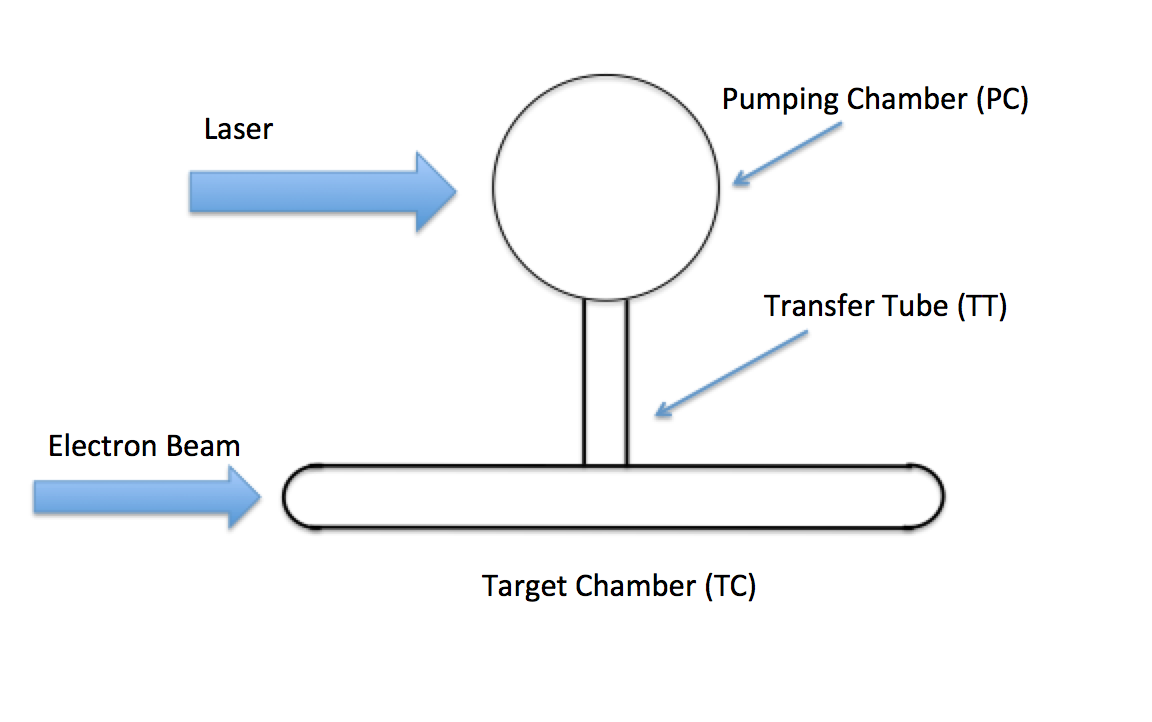
\includegraphics{TargetCell.png}}
	\caption{{ A schematic representation of a target cell. The dimensions of different parts of the cell are not to scale.}}
	\label{TargetCell}
\end{figure}

\section{New Generation Target Cells}

The future experiments planned during the 12GeV era after the upgrade will be much more demanding in terms of target cell performance. In particular, there is a desire to run experiments with higher luminosity where luminosity is the product of gas density in the target, interaction length and beam current. Increased luminosity will lead to more interactions that depolarize the target. We have designed and tested a new style cell that utilizes convection instead of diffusion to increase the rate at which the polarization in the target chamber is replenished by polarized gas from pumping chamber~\cite{PhysRevC.84.065201}. We have obtained over 50\% polarization with controllable convection speed so far.

An additional problem that comes with higher beam current is that the glass end windows of traditional design are not likely to survive the experiments. Our group started exploring the option of using metal end windows since eight years ago. Fig~\ref{metal_end_windows} shows an example configuration of such a target. The first problem to solve is to find out the correct material and the proper technique to incorporate metal without introducing significant spin relaxation and still being able to hold high pressure gas (12 atm) inside. This is a brand new technique that may have a profound impact on future cell designs once fully developed. Although no metal end windows have been tested so far, through carefully examining multiple glass cells with different kinds metal tubes (much larger in area compared to the end windows that will be used in JLAB experiments) attached, we have developed a reliable way of incorporating metal to target cells without introducing significant spin relaxation rates. We believe the next generation target cells used in the 12GeV era will be able to utilize metal end windows. In our test cells, the metals tubes were connected to Pyrex glass with Houskeeper seals~\cite{Houskeeper} and stayed intact through high pressure tests. After exploring options such as pure copper, gold coated copper, titanium, stainless steel, gold coated titanium, we have established that electroplating gold on copper substrate yields the best result so far. We have achieved a 15.6 h relaxation time with a Pyrex cell that had a 5'' long by 1'' gold coated copper tube attached horizontally. The additional relaxation rate introduced by the metal surface is proportional to the area of the gold surface. By comparing relaxation rates of test metal cells with pure-glass control cells, the relaxation rate due to the gold surface was extrapolated. With this result, we believe the relaxation rate introduced by small metal windows in a target will be less than 1/130.6 hr$^{-1}$. To the best of our knowledge, our group was the first to have proved the potential of incorporating metal to target cells in the presence of alkali vapor. 

\begin{figure}[t!]\label{metal_end_windows}
	\centering
	\resizebox{0.91\textwidth}{!}{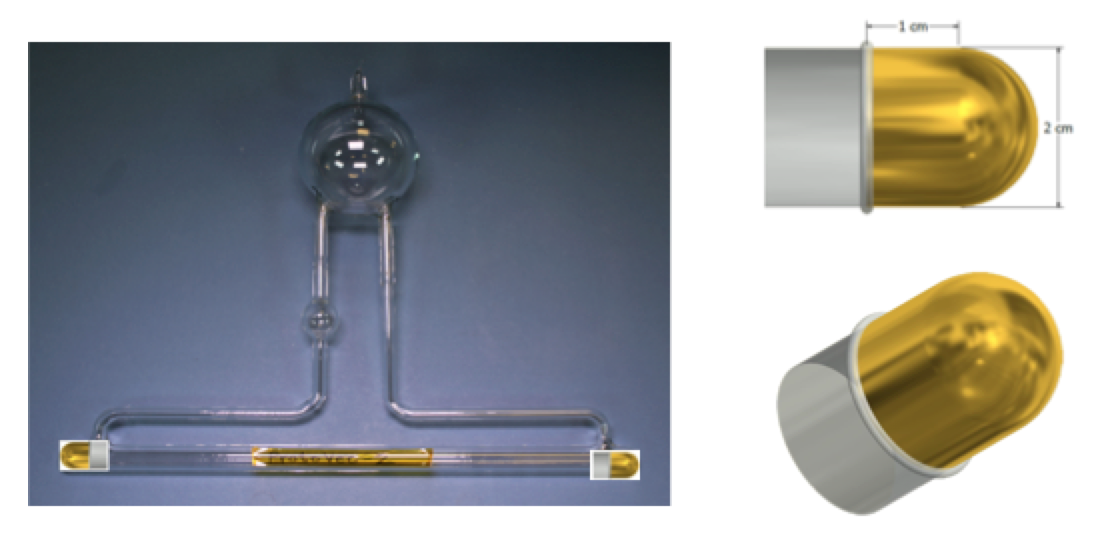
\includegraphics{metal_end_windows.png}}
	\caption{{A diagram of convection style target cell with metal end windows. }}
	\label{metal_end_windows}
\end{figure}

\section{Structure of This Thesis}

This thesis focuses on both discussion on the development of high-performance polarized $3$He targets that utilize spin-exchange optical pumping (SEOP) and the development of future target cells that incorporate metal end windows. Chapter 2 gives a general description of SEOP. Chapter 3 introduces polarimetry techniques used in our lab for target cell characterization. Chapter 4 discusses the result collected in our lab from the over-a-decade development of $^3$He target cells, in which the spin-exchange rate constant for K and $^3$He is calculated and the so-called ``X Factor" is studied. Chapter 5 presents the development process of target cells with metal parts that aims to incorporate metal end windows to future cells for the 12 GeV era experiments. Chapter 6 summarizes this thesis and suggests future directions.














\chapter{Spin-Exchange Optical Pumping}
\label{chap2}

\section{Overview}

Spin-polarized noble gases have been widely used for various purposes. In JLAB, polarized $^{3}$He is used as target for electron-scattering experiments. This is because a $^{3}$He nucleus has a pair of protons with paired spins and a single neutron that contributes the most of the nuclear spin. In MRI, polarized $^{3}$He has seen uses such as detecting structural damage in the lungs.

There are generally two ways of polarizing $^{3}$He: Metastability-Exchange Optical Pumping (MEOP) and Spin-Exchange Optical Pumping (SEOP). Our group focuses on SEOP as MEOP polarizes gas at relatively low pressure ($\sim$1 torr), thus further compression is required to produce target cells of several atms that meet the need of JLab experiments.

In SEOP, alkali metal is polarized by circularly polarized laser tuned to the D1 transition of the particular alkali species used. $^{3}$He obtains polarization from alkali metal through spin exchange process. With the combination of hybrid alkali mixtures (typically Rb and K) and spectrally narrowed lasers, more than 70\% polarizations have been produced.

\section{Optical pumping}

\subsection{Rb for SEOP}

In optical pumping, Rb is often the alkali metal chosen to be optically pumped by circularly polarized laser light. The angular momentum of a polarized photon is transfered to the valence electron of Rb atom. In the case of hybrid mixture of Rb/K, Rb is still the alkali metal that is directly pumped by laser light while K serves as an efficient medium to transfer the polarization from Rb to $^{3}$He. Because the spin destruction rates are much lower for lighter alkali metals, K-$^{3}$He spin-exchange process is a lot more efficient than that of Rb-$^{3}$He. However, it is still much easier to optically pump Rb and transfer the polarization to $^{3}$He through K, mainly for Rb's low melting point, the relative ease of acquiring laser at the Rb D1 line wavelength and the wide separation between D1 (794.7nm) and D2 line (780nm). 

The Rb melting point is at 39.5$^{\circ}$C, so it's easy to achieve enough Rb vapor without having to drive the oven temperature too high. In our lab, depending on if the cell contains pure Rb or Rb/K mixture, the oven temperature can be between 85$^{\circ}$C to as high as 255$^{\circ}$C. Perhaps the most used oven temperature for hybrid is 235$^{\circ}$C which has empirically been a good temperature to produce Rb/K mixture vapor, while 85$^{\circ}$C is enough for pure Rb.

\subsection{Vapor Pressure Curves}

When the alkali metal is heated to above its melting point, a small amount of alkali metal atoms evaporate. The equilibrium vapor pressure is temperature dependent:

\begin{equation}
P=10^{5.006+\alpha + \beta/T} Pa
\end{equation}

where $\alpha$ and $\beta$ are listed in Table~\ref{VaporPressureCoef}.

\begin{center}\label{VaporPressureCoef}
	\begin{tabular}{| l | l | l |}
		\hline
		& Patassium & Rubidim \\ \hline
		$\alpha$ & 4.402 & 4.312 \\ \hline
		$\beta$ & -4453 & -4040 \\ \hline
	\end{tabular}
\end{center}

Thus the number density is 

\begin{equation}
[A]=\frac{10^{5.006+\alpha+\beta/T}}{k_{B}T}
\end{equation}

The number density curves of pure Rb and K vapor are shown in Fig.~\ref{fig:AlkaliVaporDensity}.

\begin{figure}[t!]
	
	\centering
	\resizebox{0.91\textwidth}{!}{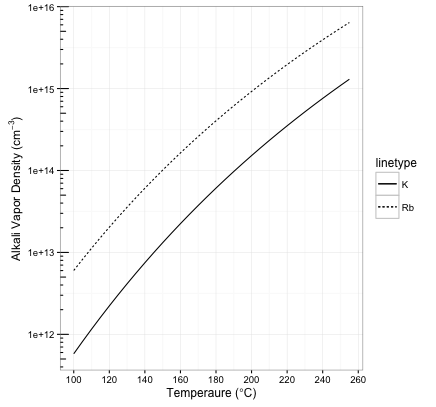
\includegraphics{AlkaliVaporDensity.png}}
	\caption[Rb And K Number Density Curves]{{\bf Rb And K Number Density Curves}}
	\label{fig:AlkaliVaporDensity}
	
\end{figure}

\subsection{Energy Levels of Alkali Metal in External Magnetic Field}

The Hamiltonian for ground state (L=0) alkali metal atoms in external magnetic field is:

\begin{equation}
{\bf H} = A{\bf I \cdot S} + g_{e} \mu_{B} S_{z}B_{z} + g_{N}{\mu_{N}}I_{z}B_{z}
\end{equation}

The first term $A{\bf I \cdot S}$ describes the coupling of the nuclear spin {\bf I} with the electron spin {\bf S} and is key to spin exchange, where A is the isotropic magnetic-dipole coupling coefficient. The resulting energy levels from the first term are referred to as hyperfine structure. The second and third terms describe the Zeeman splitting due to the presence of a weak external magnetic field. ${\mu}_{B} = 9.274 \times 10^{-24}J/T$ and ${\mu}_{N} = 5.051 \times 10^{-27}J/T$ are the Bohr and nuclear magnetons. $g_{e}\approx2$ and $g_{N}\approx5.59$ are the electronic and nuclear Lande g-factors.

The linear relationship between energy levels and magnetic field only holds for weak magnetic fields which applies to our lab where $\sim$13 Gauss is used most of the time. When the Zeeman splitting grows comparable to the hyperfine energy difference one would have to take into account the quantum mixing of the states, the result is described by Breit-Rabi Formula. With $\sim$13 Gauss, the hyperfine term dominates the total Hamiltonian. The energy levels of $^{87}$Rb are shown in Fig.~\ref{RbEnergyLevels}.

\begin{figure}[t!]
	\centering
	\resizebox{0.91\textwidth}{!}{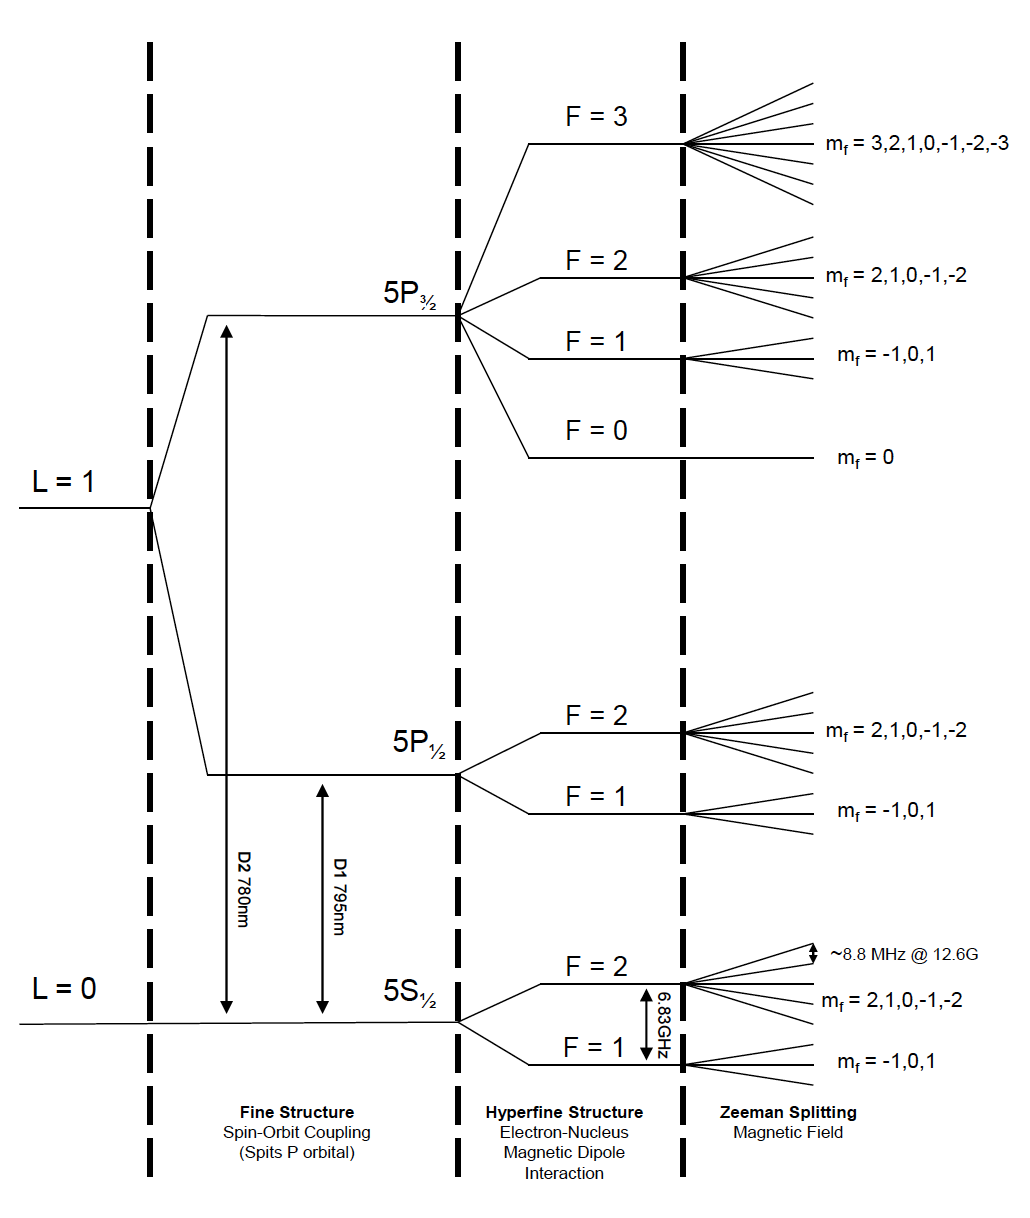
\includegraphics{RbEnergyLevels.png}}
	\caption{{\bf Level Diagram of $^{87}$Rb. The splittings are not to scale. Adapted from Dolph's PhD thesis.}}
	\label{RbEnergyLevels}
\end{figure}

\subsection{Optical Pumping Process Overview}

For simplicity, the following discussion will ignore the nuclear spins for now. The inclusion of nuclear spins will increase the number of energy states but the optical pumping mechanism remains the same. In our typical setup, circularly polarized laser light is tuned to the D1 line of Rb and excites valence electrons of Rb from 5S$_{1/2}$ state to 5P$_{1/2}$ state as shown in Fig.~\ref{fig:OpticalPumping} (2S$_{1/2}$ and 2P$_{1/2}$ states are used in the simple model described by the figure below). 

\begin{figure}[t!]
	\centering
	\resizebox{0.91\textwidth}{!}{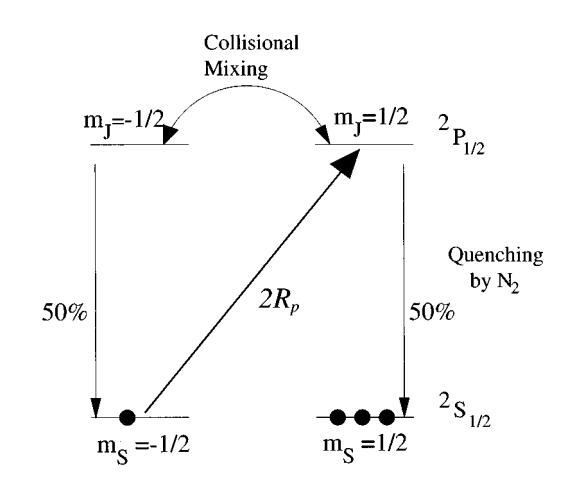
\includegraphics{OpticalPumping.png}}
	\caption{{\bf The interaction of alkali-metal atoms with left-circularly ($\sigma^{+}$) polarized light. (from Ref.\@ \cite{WalkerHapper})}}
	\label{fig:OpticalPumping}
\end{figure}

Left-circularly polarized light is assumed in the figure, but either circular polarization works the same. Conservation of angular momentum requires $\Delta$m = +1 as the figure shows. Through collisions with other Rb atoms, excited electrons will mix and evenly distribute on the two 2P$_{1/2}$ states. Electrons then decay to the two ground states with equal probabilities. The selection rule for the decay process is $\Delta$m = 0 or $\pm$1. Even though both ground states receive electrons from the decay, only the m = -1/2 state absorbs the circular polarized photons and is being depleted, so atoms are in effect pumped to the m = +1/2 state. When we consider Rb with nuclear spins, both 5S$_{1/2}$ and 5P$_{1/2}$ states are split into more energy levels, but the net effect is still that the ground state with highest m accumulate atoms over time.

When the excited electrons decay back to the ground state, they emit unpolarized photons with angular momentum in random directions which can depolarize the gas. A small amount of N$_{2}$ gas is added into the cell (typically around 0.1 Amagats) to non-radiatively quench the excited electrons as N$_{2}$ molecules can absorb the released energy of spontaneous decays into their rotational and vibrational modes of oscillation. With an appropriate amount of N$_{2}$, the photon-emitting decays can be reduced to less than 5\%.

\subsection{Optical Pumping Rate}

The optical pumping rate at position $\vec{r}$ can be described by

\begin{equation}
R = \int \Phi(\nu, \vec{r})\sigma(\nu)d\nu
\end{equation}

where $\Phi(\nu,\vec{r})$ is the position dependent photon spectral flux density and $\sigma(\nu)$ is the photon absorption cross section. The cross section has a natural Lorentzian lineshape which is broadened by Doppler effect and pressure broadening. The pressure broadening effect dominates the lineshape as our cells normally have densities well above one amagat. The collisions of Rb with $^{3}$He and N$_{2}$ cause the broadening as well as a slight shift of the D$_{1}$ line. The coefficients of pressure broadening for $^{3}$He, $^{4}$He and N$_{2}$ are listed in Table~\ref{PBCoef}, and can be used to calculate the broadened line width and the shifted line center.

\begin{center}\label{PBCoef}
	\begin{tabular}{ c c c c c c}
		\hline \hline
		& $^{4}$He & $^{3}$He & Temp. depen. & N$_{2}$ & Temp. depen.\\ 
		D$_{1}$ full width & 18.0$\pm$0.2 & 18.7$\pm$0.3 & T$^{0.05\pm0.05}$ & 17.8$\pm$0.3 & T$^{0.3}$\\ 
		(GHz/amg) &&&&& \\
		D$_{1}$ line shift & 4.3$\pm$0.1 & 5.64$\pm$0.15 & T$^{1.1\pm0.1}$ &
		-8.25$\pm$0.15 & T$^{0.3}$ \\ 
		(GHz/amg) &&&&& \\ \hline \hline
	\end{tabular}
\end{center}

\begin{figure}[t!]
	\centering
	\resizebox{0.91\textwidth}{!}{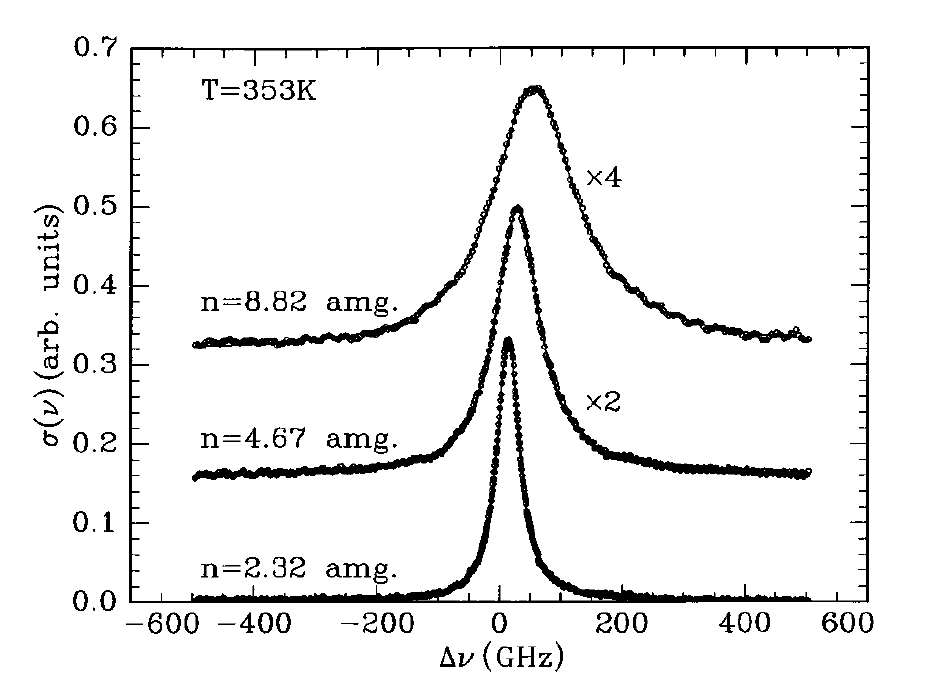
\includegraphics{AbsorptionLine.png}}
	\caption{{\bf Absorption cross section for Rb $D_{1}$ line in the presence of three different densities of $^{3}$He. (from Ref.\@ \cite{Romalis1997})}}
	\label{AbsorptionLine}
\end{figure}

\begin{figure}[t!]
	\centering
	\resizebox{0.91\textwidth}{!}{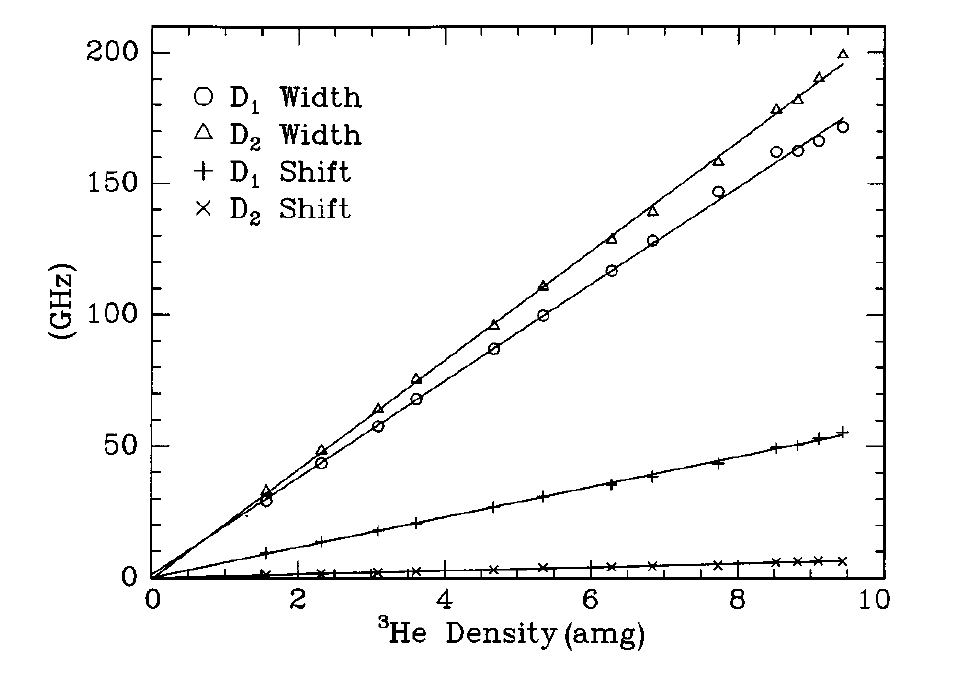
\includegraphics{PressureBroadening.png}}
	\caption{{\bf The shift and the broadening due to presence of $^{3}$He for Rb $D_{1}$ and $D_{2}$ lines. (from Ref.\@ \cite{Romalis1997})}}
	\label{PressureBroadening}
\end{figure}

$\sigma(\nu)$ follows the sum rule:

\begin{equation}
\int\sigma(\nu)d\nu=\pi r_{0}cf
\end{equation}

where $r_{0}=2.82 \times 10^{-13}$ cm is the classical electron radius and f=0.337is the transition oscillator strength. Thus the photon absorption cross section can be described by Lorentzian lineshape:

\begin{equation}
\sigma(\nu)=fr_{e}c\frac{\frac{\Gamma_{A}}{2}}{(\nu-\nu_{0})^{2}+(\frac{\Gamma_{A}}{2})^{2}}
\end{equation}

where $\Gamma_{A}$ is the pressure dependent FWHM, $\Gamma_{A}\approx 0.04nm/amg \cdot [^{3}He]$. At the front of the cell, the photon spectral flux density is the product of a Gaussian spatial distribution and a Gaussian spectrum.

\begin{subequations}
	\begin{gather}
	\phi(\nu,\vec{r})=\phi_{0}(\vec{r})G(\nu) \\
	\phi_{0}(\vec{r})=\frac{P}{h\nu}\frac{2}{\omega^{2}\pi}e^{2r^{2}/\omega^{2}}\\
	G(\nu)=\frac{1}{\sqrt{2\pi}\sigma_{l}}e^{-(\nu-\nu_{l})^2/2\sigma_{l}^{2}}
	\end{gather}
\end{subequations}

where P is the laser power; $\omega$ is the beam waist;  $\sigma_{l}$ is the Gaussian width of the laser and $\nu_{l}$ is the central laser frequency.

\subsection{Polarization Time Evolution}

Polarizations of Rb electrons are more complex, but $^{3}He$ nuclei have an intrinsic nuclear spin of 1/2, and it is simpler to explain the math with spin of 1/2. Let's define the polarization as the asymetry between +1/2 state and -1/2 state:

\begin{equation}
P=\frac{\rho_{+1/2}-\rho_{-1/2}}{\rho_{+1/2}+\rho_{-1/2}}=\rho_{+1/2}-\rho_{-1/2}
\end{equation}

where $\rho_{\pm 1/2}$ is the population in the $\pm1/2$ state.

The time evolution of polarization for both Rb electrons and $^{3}He$ follows the equation:

\begin{equation}
\frac{dP}{dt}=\gamma(1-P)-\Gamma \cdot P
\end{equation}

$\gamma$ is the polarization rate and $\Gamma$ is the depolarization rate in the above differential equation. The solution has the simple form of:

\begin{equation}
P(t)=Ce^{-(\gamma+\Gamma)t} + \frac{\gamma}{\gamma+\Gamma}
\end{equation}

Note the depolarization rate also contributes to the rate at which P approaches saturation as it lowers the saturated polarization hence shortens the time to reach it. The saturated polarization is defined as the value of P in the limit t $\rightarrow \infty$:

\begin{equation}
P_{\infty}=\frac{\gamma}{\gamma+\Gamma}
\end{equation}

The initial polarization is defined as the value of P at t = 0:

\begin{equation}
P_{0}=C+\frac{\gamma}{\gamma+\Gamma}=C+P_{\infty}
\end{equation}

Thus, P(t) can be expressed as:

\begin{equation}
P(t)=(P_{0}-P_{\infty})e^{-(\gamma+\Gamma)t}+P_{\infty}
\end{equation}

In the case of polarizing Rb with a pump laser, $\gamma$ is the pumping rate R and $\Gamma$ is the Rb spin relaxation rate $\Gamma_{Rb}$. There is typically a small angle $\theta$ between the pump laser and the holding field even though great effort has been made to minimize the angle. Thus P(t) can be rewritten as:

\begin{equation}\label{Pt}
P(t) = P_{0}e^{-(R+\Gamma_{Rb})t} + P_{laser}cos\theta \frac{R}{R+\Gamma_{Rb}}(1-e^{-(R+\Gamma_{Rb})t})
\end{equation}

$P_{laser}$ is the circular polarization of the pump laser which is above 99.5\%. Rb close to the front side of the cell can reach above 97\% (depends on the laser power and other factors) on the order of 100's of microseconds. As the laser propagates through the cell, power is attenuated by Rb vapor. Therefore Rb polarization at the back side of the cell is lower than that at the front side. One way to overcome the problem is to shine pump laser from both sides of the cell which would lead to higher overall Rb polarization and $^{3}$He polarization.

Spins are thermally polarized with the presence of a magnetic field even without external pumping source. The probability for a spin to be in state s is:

\begin{equation}
Prob. = \frac{e^{-E_{s}/k_{B}T}}{\sum_{si}e^{-E_{si}/k_{B}T}}
\end{equation}

where $E_{s}$ is the energy of the state, $k_{B}$ is the Boltzmann constant and T is the temperature. Using the thermal distribution, under typical operating conditions, $^{3}He$ polarization is ~$10^{-9}$ and Rb polarization is ~$10^{-5}$. Both are negligible without active pumping.

\subsection{Rb Spin Destruction Rate}

There are two main mechanisms of Rb depolarization: the binary collisions with Rb, $^{3}$He and $N_{2}$, and the formation and breakup of van der Waals molecules, the second mechanism is negligible for $^{3}$He cells. The Rb spin destruction rate can then be expressed as

\begin{equation}
\Gamma_{Rb}=k_{Rb-Rb}[Rb]+k_{Rb-^{3}He}[^{3}He]+k_{Rb-N_{2}}[N_{2}]
\end{equation}

where $k_{Rb-X}$ is the spin destruction rate constant and [X] is the density of X. Dolph has summarized these constants based on measurements from various groups:

\begin{subequations}
	\begin{gather}
	k_{Rb-^{3}He}(T)=55.9(9)\left(\frac{T}{473.15K}\right)^{3.31(12)}Hz/amg\\
	k_{Rb-N_{2}}(T)=290(30)\left(\frac{T}{473.15K}\right)^{2.0(25)}Hz/amg\\
	k_{Rb-Rb}=4.813(48)\times 10^{-13}Hz\cdot cm^{3}
	\end{gather}
\end{subequations}

For a pure Rb cell at 170$^{\circ}$C with the following densities in the pumping chamber:

\begin{subequations}
	\begin{gather}
	[^{3}He] \approx 8.0 amg\\
	[N_{2}] \approx 0.08 amg\\
	[Rb] \approx 6.0 \times 10^{14} cm^{-3}
	\end{gather}
\end{subequations}

The approximate spin destruction rates due to various gases are:

\begin{subequations}
	\begin{gather}
	\Gamma_{Rb-^{3}He} \approx 360Hz\\
	\Gamma_{Rb-N_{2}} \approx 20Hz\\
	\Gamma_{Rb-Rb} \approx 289Hz
	\end{gather}
\end{subequations}

The total spin destruction rate is 669 Hz.

\section{Spin Exchange}

Following equation \ref{Pt}, the time evolution of $^{3}He$ polarization can be expressed as:

\begin{equation}
P_{^{3}He}(t) = P_{0}e^{-(\gamma_{se}+\Gamma)t} + P_{Rb} \frac{\gamma_{se}}{\gamma_{se}+\Gamma}(1-e^{-(\gamma_{se}+\Gamma)t})
\end{equation}

The saturation polarization is 

\begin{equation}
P_{\infty} = P_{Rb}\frac{\gamma_{se}}{\gamma_{se}+\Gamma}
\end{equation}

where $\gamma_{se}$ is the spin exchange rate between $^{3}$He and Rb, and $\Gamma$ is the spin relaxation rate. 

\subsection{Spin-Dependent Interactions}

The key process in spin-exchange optical pumping is collisional transfer of polarization between optically pumped alkali-metal atoms and the nuclei of the noble gas atoms. As in Fig. \ref{SpinExchange}, the transfer of angular momentum occurs either while the atoms are bound in van der Waals molecules or in simple binary collisions. For $^{3}He$, binary collisions dominate, and the contribution from van der Waals molecules is negligible. The time scale for binary collisions is on the order of $~10^{-12}$ sec, so the collision can induce both $\Delta F=\pm1$ and $\Delta F=0$ transitions between hyperfine sublevels. For heavier noble gases like $^{129}$Xe at pressure of a few tens of Torr, the contributions of van der Waals molecuels can greatly exceed that of binary collisions. At several atms which is the typical operating pressure for SEOP, the time scale of van der Waals molecules is greatly limited by collision so that the binary collisions dominate.

\begin{figure}[t!]
	\centering
	\resizebox{0.91\textwidth}{!}{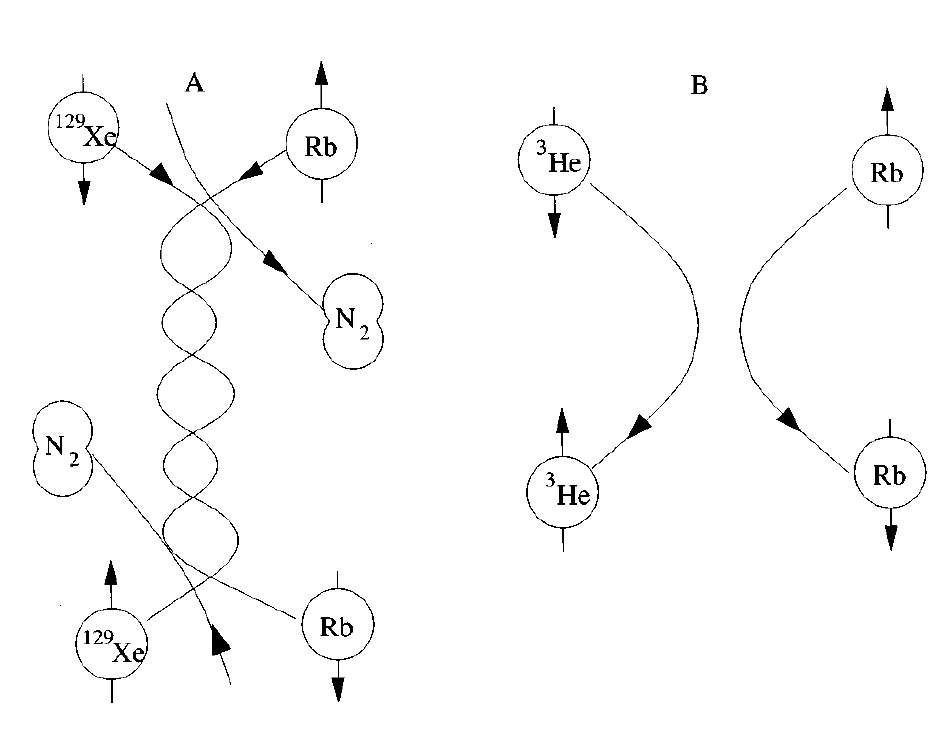
\includegraphics{SpinExchange.png}}
	\caption{{\bf A. Formation and breakup of alkali-metal/noble-gas van der Waals molecule. B. Binary collision between an alkali-metal atom and a noble-gas atom. (from Ref.\@ \cite{WalkerHapper})}}
	\label{SpinExchange}
\end{figure}

Spin-dependent interactions produce the spin transfer and relaxation. For SEOP, spin-rotation interaction between $\vec{S}$ and the rotational angular momentum $\vec{N}$ and the isotropic hyperfine interaction between $\vec{S}$ and the noble-gas nuclear spin $\vec{I}$ dominate the spin-exchange process:

\begin{equation}\label{V1}
V_{1}(\vec{R})=\gamma(R)\vec{N}\cdot \vec{S}+A(R)\vec{I}\cdot \vec{S}
\end{equation}

$\vec{I}_{a}$ and $\vec{I}_{b}$ are the nuclear spins of the atomic pair.

The spin-rotation interaction is caused by the magnetic fields from relative motion of the charges of the colliding atoms, and the isotropic hyperfine interaction comes from the magnetic field inside the nucleus of the noble-gas atom. 

An alkali-metal atom and a noble-gas atom interact via both a large spin-independent interaction $V_{0}(R)$ and a small spin-dependent interaction $V_{1}(R)$. At the high operating temperatures, $V_{0}$ determines classical collision trajectories, while $V_{1}$ acts as a small perturbation. We'll focus on $V_{1}$ below since it is responsible for spin exchange.

Including a few more terms that were neglected in Eq. \ref{V1}, the spin-dependent interaction $V_{1}(R)$ can be expressed as:

\begin{equation}
\begin{split}
V_{1}(\vec{R})=\gamma(R)\vec{N}\cdot \vec{S}+\sum_{k}A_{k}(R)\vec{I}_{k}\cdot \vec{S}\\
+\sum_{k}B_{k}(R)\vec{I}_{k}\cdot (3\vec{R}\vec{R}-1)\cdot \vec{S}\\
+\sum_{k}C_{k}(R)\vec{I}_{k}\cdot (3\vec{R}\vec{R}-1)\cdot \vec{I}_{k}
\end{split}
\end{equation}

\begin{figure}[H]
	\centering
	\resizebox{0.91\textwidth}{!}{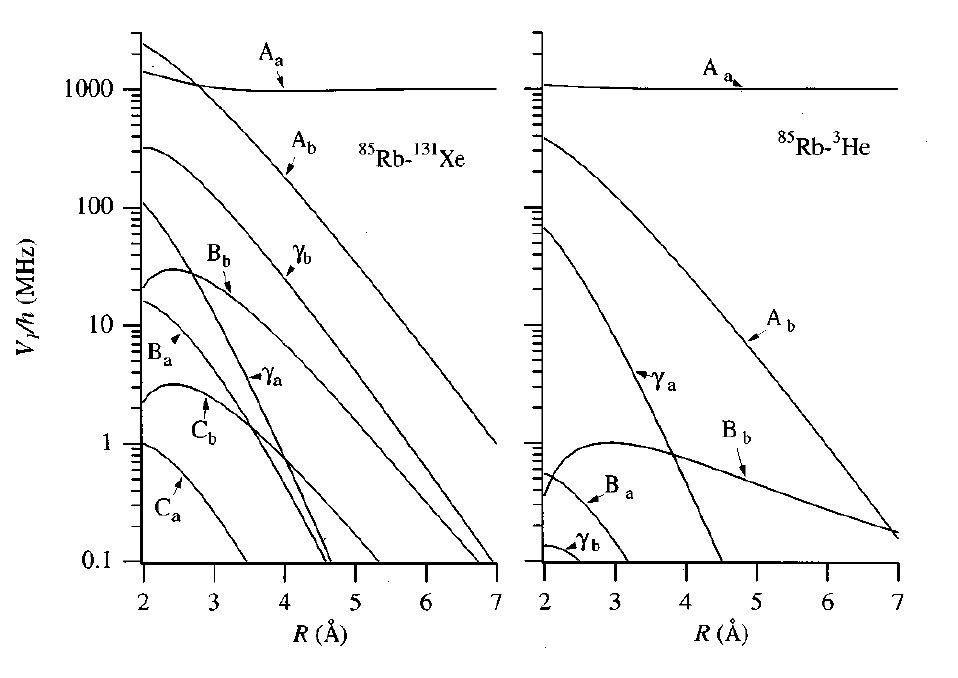
\includegraphics{V1.png}}
	\caption{{\bf Strengths of various spin-dependent interactions as functions of separation(from Ref.\@ \cite{WalkerHapper})}}
	\label{SpinExchange}
\end{figure}

where $\gamma$ is the coefficient of the spin-rotation interaction, while $A_{k}$, $B_{k}$, $C_{k}$ are the coefficients for isotropic magnetic-dipole hyperfine interactions, anisotropic magnetic-dipole hyperfine interactions, and electric quadrupole interactions, respectively. $A_{a}$ greatly exceed other coefficients as the separations between atoms increase. 

The isotropic hyperfine interactions come from the Fermi-contact magnetic fields of the nuclei pair. 

\begin{equation}
A_{b}(R)=\frac{8\pi g_{s}\mu_{B}\mu_{b}}{3I_{b}}|\eta \phi_{0}(R)|^{2}
\end{equation}

where $\eta$ is the enhancement factor which equals to the ratio of the perturbed wave function at the noble gas nucleus to that without the noble gas atom. The isotropic hyperfine interaction also introduces a frequency of the magnetic resonance lines for alkali-metal and noble gas atoms. The frequency shift of alkali-metal electrons due to the polarized noble gas nuclei is used in the technique Electron Paramagnetic Resonance (EPR) to calculate the polarization of noble gas nuclei.

The isotropic magnetic-dipole coupling polarizes the noble gas nuclei parallel to the electron spin polarization, while the anisotropic magnetic-dipole coupling polarizes in the opposite direction. Fortunately, the anisotropic interaction is negligible compared to isotropic interaction.

\subsection{Spin Exchange Rate}

The spin exchange rate due to binary collisions is:

\begin{equation}
\gamma_{se}=<\sigma_{se}v>[Rb]=k_{se}[Rb]
\end{equation}

where $k_{se}=<\sigma_{se}v$ is the velocity-averaged spin exchange rate constant. $k_{se}$ for spin exchange between $^{3}He$ and Rb is:

\begin{equation}
k_{se}^{^{3}He-Rb}=(6.7\pm 0.7)\times 10^{-20}cm^{3}/s
\end{equation}

Under 170$^{\circ}$C which is a typical temperature that we run tests with,

\begin{equation}
[Rb]=2.60\times 10^{14}cm^{-3}
\end{equation}

Thus for a single chamber cell,

\begin{equation}
frac{1}{\gamma_{se}}\approx 15.9 hrs
\end{equation}

\section{$^{3}He$ Spinup and Relaxation}

Similar to the optical pumping process of Rb, $^{3}He$ polarization can be described by

\begin{equation}
P_{^{3}He}(t)=P_{0}^{^{3}He}e^{-(\gamma_{se}+\Gamma)t}+P_{\infty}^{^{3}He}(1-e^{-(\gamma_{se}+\Gamma)t})
\end{equation}

where the saturation polarization is

\begin{equation}
P_{\infty}^{^{3}He}=P_{\infty}^{Rb}\frac{\gamma_{se}}{\gamma_{se}+\Gamma}
\end{equation}

And $\Gamma$ is the total relaxation rate of $^{3}$He nucleus spin polarization,

\begin{equation}
\Gamma=\Gamma_{dipolar}+\Gamma_{inhomogeneity}+\Gamma_{wall}
\end{equation}

When a target cell are used in electron scattering experiments where an electron beam goes through part of the cell, an additional relaxation rate due to the beam $\Gamma_{beam}$ should also be included.

The coupling of nuclear spin to orbital angular momentum creates an intrinsic $^{3}$He relaxation rate that depends on density. At room temperature (23$^{\circ}C$), the dipolar relaxation rate is 

\begin{equation}
\frac{1}{\Gamma_{dipolar}}=\frac{[^{3}He]}{744}hr^{-1}
\end{equation}


where [$^{3}He$] is the $^{3}He$ density in amagats. Assuming the cell density is 8 amg, the relaxation rate is 1/93 $hr^{-1}$. In addition, there is an additional intrinsic relaxation due to the spin-rotation interaction. This mechanism dominates the relaxation for $^{129}$Xe but is small for $^{3}$He. 

The relaxation rate due to field inhomogeneities is

\begin{equation}
\Gamma_{inhomogeneity} = D\frac{|\nabla B_{x}|^{2}+|\nabla B_{y}|^{2}}{B_{0}^{2}}
\end{equation}

where D is the $^{3}$He diffusion constant, $\nabla B_{x}$ and $\nabla B_{y}$ are the transverse magnetic field inhomogeneities, $B_{0}$ is the holding field along z-axis. Under operating conditions, assuming the pressure is around 12 atm and field is 12.6 G, $D\approx 0.16cm^{2}/s$ and the field inhomogeneities are ~ 10mG/cm, the relaxation rate is ~ 1/1400 hr$^{-1}$

Wall relaxation is typically the dominant relaxation mechanism for cells in our lab. This mechanism depends on the property of the inner surface of glass. Most of the target cells are contructed with reblown General Electric Type 180 (GE-180) glass. This aluminosilicate glass is highly impermeable to $^{3}$He. The wall relaxation is believed to be associated to several different mechanisms, such as paramagnetic impurities in the glass and microfissures in the surface that could trap $^{3}$He atoms. It has been found reblowing the glass can help lower the wall relaxation rate because it reduces the number of microfissures. The wall relaxation is not well understood, but it is believed to scale with the surface-to-volume ratio:

\begin{equation}
\Gamma_{wall} = \rho S/V
\end{equation}

where $\rho$ is called relaxivity.

\section{X Factor}

In 2006, Babcok \emph{et al.} reported evidence of a previously unrecognized spin relaxation mechanism, and named it X factor. This mechanism appears to be temperature dependent and roughly proportional to alkali density. The X factor limits the maximally achievable $^{3}$He polarization even with infinite laser power. The saturation polarization is 

\begin{equation}
P_{\infty}^{^{3}He}=P_{\infty}^{Rb}\frac{\gamma_{se}}{\gamma_{se}(1+X)+\Gamma}
\end{equation}

In the presence of infinite laser power where $\gamma_{se} \gg \Gamma$, the saturation polarization becomes

\begin{equation}
P_{\infty}^{^{3}He}=P_{\infty}^{Rb}\frac{1}{1+X}
\end{equation}



















\chapter{$^{3}$He Polarimetry}
\label{chap:chap3}

\section{Overview}

Traditional pure glass target cells are studied mainly using Adiabatic Fast Passage (AFP) Nuclear Magnetic Resonance (NMR) and Electron Paramagnetic Resonance (EPR). AFP is a technique that allows us to monitor a signal that's directly proportional to the ${3}He$ polarization, which then provides a means to gain knowledge of properties of cell including pumping time and relaxation rates. The EPR technique utilizes the fact that polarized $^{3}$He produces frequency shift of the magnetic resonance lines of alkali metal to measure the $^{3}$He polarization. When AFP and EPR are combined, we can calculate the calibration constant between AFP signal and $^{3}$He polarization. 

A significant focus of my studies is on exploring cells that incorporate metal. Unfortunately, AFP is not suitable for studying these cells as it requires exposing the entirety of the cell to a Radio Frequency magnetic field in an attempt to flip all spins in the cell. For these cells, Pulsed Nuclear Magnetic Resonance (PNMR) has proven to be very useful. PNMR only applies a pulsed RF field to a small selected part of the cell which makes it relatively easy to prevent metal from distorting the signal. However, the spins tipped by applying the pulse lose their transverse component (which depends on the "tip angle"), we typically allow some time for this portion of gas to diffuse out of the region before taking the next measurement on a fresh sample of the gas. The rate at which measurements are taken is limited by this requirement.

This chapter introduces the three techniques mentioned above and how they're used for our studies.

\section{Adiabatic Fast Passage}

\subsection{Nuclear Magnetic Resonance}

The energy of a magnetic moment in an external field is

\begin{equation}
E = -\vec{\mu}\cdot \vec{B_{0}} = -\mu_{z}B_{0}
\end{equation}

where $\vec{\mu}$ is the magnetic moment, for a spin-1/2 nuclei, the energy is

\begin{equation}
E = -\gamma B_{0}\hbar/2
\end{equation}

$\gamma$ is the gyromagnetic ratio, $\gamma /2\pi \approx 3.2434kHz/Gauss$. When a oscillating magnetic field with the frequency $\omega=\gamma B_{0}$ is present, transitions between the +1/2 and -1/2 states are induced. This frequency is called Larmor frequency. When a nucleus is placed in an external magnetic field that is not aligned with its magnetic moment, it will precess at the Larmor frequency.

\subsection{The Rotating Coordinate System}

\subsubsection{Classical Formulation}

For a nucleus in an external field $\vec{B}$ with $\gamma \hbar \vec{I}$ as its nuclear angular momentum, the equation of motion in a stationary coordinate system is \cite{RevModPhys.26.167}

\begin{equation}\label{eq1}
\hbar \frac{d\vec{I}}{dt}=\gamma \hbar \vec{I} \times \vec{B}
\end{equation}

Let $\frac{\partial}{\partial t}$ represent the derivative with respect to a coordinate system that rotates with angular velocity $\vec{\omega}$,

\begin{equation}{eq2}
\frac{d\vec{I}}{dt}=\frac{\partial \vec{I}}{\partial t}+\vec{\omega} \times \vec{I}
\end{equation}

Substitute Eq.\@ \ref{eq2} into Eq.\@ \ref{eq1}, $\vec{I}$ in the rotating frame satisfies the equation of motion 

\begin{equation}
\hbar \frac{\partial \vec{I}}{\partial t}=\gamma \hbar \vec{I} \times (\vec{B} + \vec{\omega}/\gamma)=\gamma \hbar \vec{I} \times \vec{B_{eff}}
\end{equation}

where $\vec{B_{eff}}$ is the effective field in the rotating frame

\begin{equation}
\vec{B_{eff}}=\vec{B} + \vec{\omega}/\gamma
\end{equation}

Thus, for an observer in the rotating frame, the net effect is the same as changing the field to include an additional term $\omega/\gamma$.

If we apply this result to rotating magnetic fields, we will get the core idea of performing an Adiabatic Fast Passage (AFP) measurement. Assuming a constant field $\vec{B}$ and another field $\vec{B_{1}}$ perpendicular to $\vec{B}$ and rotates with angular velocity $-\omega$. In the rotating frame that rotates with $\vec{B_{1}}$, both aforementioned field are constant. The effective field in the rotating frame is

\begin{equation}\label{EffectiveField}
B_{eff}\vec{z}=(B-\omega/\gamma)\vec{z} + B_{1}\vec{x'}
\end{equation}

where $\vec{x'}$ is the direction that $\vec{B_{1}}$ is in. When on resonance (B = $\omega/\gamma$), the effective field is perpendicular to the constant field $\vec{B}$.

\subsubsection{Quantum Mechanical Formulation}

The Shr$\ddot{o}$dinger equation for a magnetic moment in an external field is

\begin{equation}\label{eq3}
i\hbar \dot{\psi}=\mathcal{H} \psi=-\gamma \hbar \vec{I}\cdot \vec{B} \psi
\end{equation}

Let $\psi$ and $\vec{B}$ be the wave function and magnetic field in a stationary frame and $\psi_{r}$ and $\vec{B_{r}}$ be the same quantities in a rotating frame with angular velocity $\vec{\omega}$. Using the rotation operator in quantum mechanics, 

\begin{subequations}\label{eq4}
	\begin{gather}
	\psi=e^{-i\vec{\omega}\cdot \vec{I}t}\psi_{r} \\
	\vec{I}\cdot \vec{B_{r}} = e^{i\vec{\omega}\cdot \vec{I}t}\vec{I}\cdot \vec{B} e^{-i\vec{\omega}\cdot \vec{I}t}
	\end{gather}
\end{subequations}

Substituting \ref{eq3} into Eq.\ref{eq3}, the Shr$\ddot{o}$dinger equation in the rotating frame is obtained

\begin{equation}
i\hbar \dot{\psi_{r}}=-\gamma \hbar \vec{I}\cdot(\vec{B_{r}} + \vec{\omega}/\gamma)\psi_{r}=-\gamma \hbar \vec{I}\cdot\vec{B_{eff}}\psi_{r}
\end{equation}

The same effective field in the rotating frame is reached as that from the classical derivation.

\subsection{Adiabatic Fast Passage}

Adiabatic Fast Passage (AFP) NMR is used to measure the $^{e}$He polarization. In an AFP measurement, with the assistance of a oscillating radiofrequency (RF) field, the spins follow the effective field in a rotating frame (as discussed in more detail below) and are flipped 180 degrees to the opposite direction and then flipped back, producing two peaks in signal when they're perpendicular to the pick up coils.

The flipping process can be achieved by either sweeping the main holding field or sweeping the RF frequency so that the longitudinal component of effective field in the rotating field goes through zero. AFP measurements in out lab are typically done by sweeping the holding field while keeping the RF frequency constant. The RF coils produce a RF field of magnitude 2$B_{1}$ perpendicular to the main holding field B. The oscillating field has a frequency of $\omega$ and can be decomposed into two counter-rotating components with the same amplitude B$_{1}$. Only the component rotating in direction to be able to give a resonance in Eq.\ref{EffectiveField} has an important effect. In this frame, the effective field is

\begin{equation}
B_{eff}\vec{z}=(B-\omega/\gamma)\vec{z} + B_{1}\vec{x'}
\end{equation}

as discussed above. The other rotating component does not affect the spins. In an AFP measurement, the holding field starts from a value that's lower than $\omega/\gamma$ ($\omega/\gamma-B\gg B_{1}$), so that the effective field is almost aligned with the holding field (and the spins). The holding field is then swept at a constant rate through resonance to a value greater than $\omega/\gamma$. The sweeping rate is of great importance. The sweep needs to be slow enough so that the nuclear spins can follow the effective field

\begin{equation}
\frac{\dot B}{B_{1}}\ll \omega
\end{equation}

Sweep that satisfies this condition is considered as adiabatic.

Sweep rate cannot be too slow either, because the relaxation rate of the spins are faster near the resonance especially with a small effective field. The relaxation rate of $^{3}$He in the rotating frame at resonance is 

\begin{equation}
\frac{1}{T_{1r}}=D\frac{|\nabla B_{z}|^{2}}{B_{1}^{2}} 
\end{equation}

where D is the $^{3}$He diffusion constant. In order to keep the AFP loss low, it's important for the time scale that the spins stay close to resonance to be much shorter than $1/T_{1r}$:

\begin{equation}
D\frac{|\nabla B_{z}|^{2}}{B_{1}^{2}} \ll \frac{\dot B}{B_{1}}
\end{equation}

Typically, the field is swept from 12.6 Gauss to 20.4 Gauss in 6s, thus

\begin{subequations}
	\begin{gather}
	\dot B = 1.3G/s\\
	B1 \approx 100mG\\
	f = 56.6kHz\\
	D \approx 0.16cm^2/s\\
	|\nabla B_{z}| \approx 10mG/cm\\
	\end{gather}
\end{subequations}

With these operating conditions, 

\begin{subequations}
	\begin{gather}
	D\frac{|\nabla B_{z}|^{2}}{B_{1}^{2}} \approx 1.6mHz\\
	frac{\dot B}{B_{1}} \approx 13Hz\\
	w \approx 356kHz
	\end{gather}
\end{subequations}

The AFP conditions are clearly well satisfied. Fig.\ref{AFP} shows the evolution of effective field during an AFP measurement.

\begin{figure}[H]
	\centering
	\resizebox{0.91\textwidth}{!}{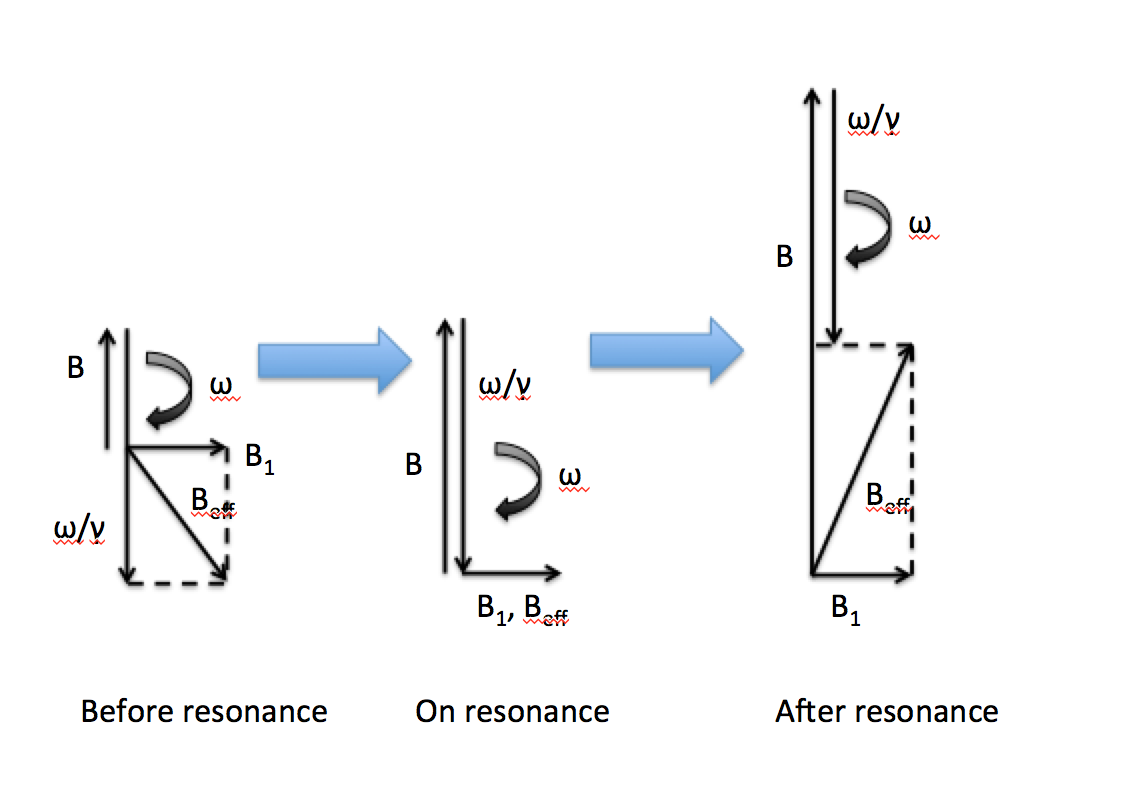
\includegraphics{AFP.png}}
	\caption{{\bf Effective field in the rotating frame during an Adiabatic Fast Passage measurement. The $^{3}He$ spins follow the direction of the effective field. $B_{1}$ is exaggerated to show different components of effective field clearly.}}
	\label{AFP}
\end{figure}

The pick up coils are placed close to the cell and perpendicular to the holding field and RF field. As the $^{3}$He spins precess along the holding field, the transverse component of the spins will induce an electromotive force (EMF) that is directly proportional to the amplitude of the component in the pick up coils. The signal can be written as:

\begin{equation}
S=A\omega \sin{\alpha(t)}=A\omega \frac{B_{1}}{B_{1}^{2}+(B(t)-\omega/\gamma)^{2}}
\end{equation}

where A is a constant that accounts for the cell and coils geometry, the cell magnetization and the electronics factors that affect the size of signal; $\omega$ is the RF frequency; $\alpha$ is the angle between the effective field and the holding field in the rotating frame; B(t) is the holding field as a function of time. The signal reaches peak value when B(t) = $\omega/\gamma$. Fig.\ref{AFPSignal} shows the result of a typical AFP measurement.

\begin{figure}[H]\label{AFPSignal}
	\centering
	\resizebox{0.91\textwidth}{!}{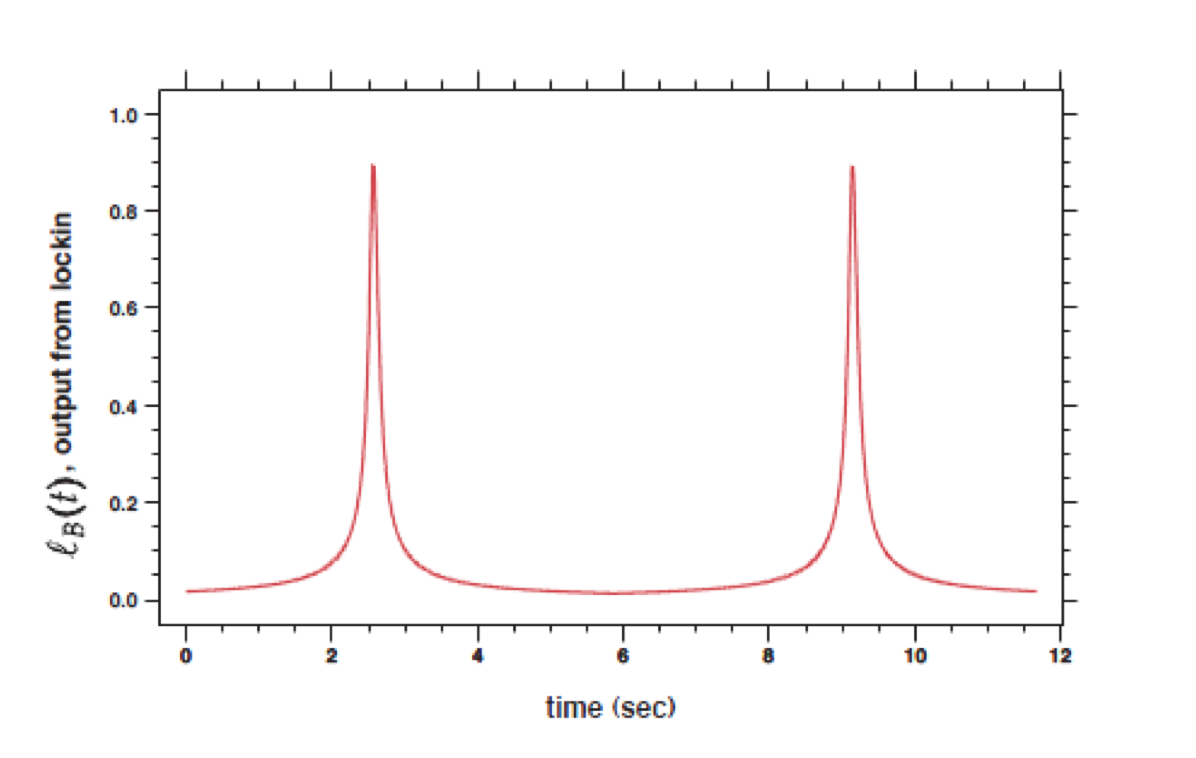
\includegraphics{AFPSignal.png}}
	\caption{{\bf A typical AFP signal. y axis is in arbitrary unit.}}
	\label{AFPSignal}
\end{figure}

\subsection{Spinups and Spindowns}

As previously mentioned, AFP is used to monitor the polarization of $^{3}$He. An exact value of polarization remains to be calibrated with EPR, but the signal size is directly proportional to the polarization, thus is an indication of how the polarization changes relatively. Two processes that are monitored with AFP are spinups and spindowns. 

\subsubsection{Double-Chambered Cell Spinup}

The process of $^{3}$He gaining polarization through spin-exchange with Rb that are being constantly pumped by circularly polarized laser is called spinup. The equation that describes spinups of single-chambered cell was already discussed in Chapter 2. But target cells used in electron-scattering experiments are normally composed of two chambers: a pumping chamber (PC), which is placed in an oven and pumped by circularly polarized laser, and a target chamber (TC) that the electron beam passes through. Fig.\ref{TargetCell} shows a typical cell.

\begin{figure}[H]
	\centering
	\resizebox{0.91\textwidth}{!}{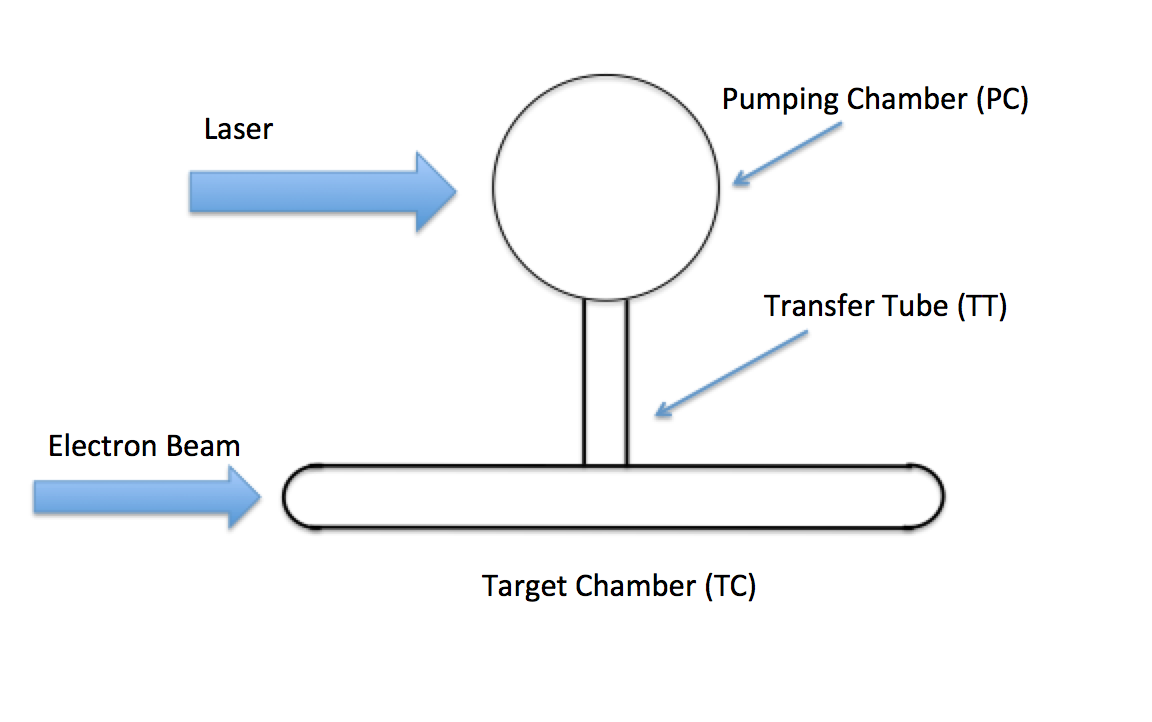
\includegraphics{TargetCell.png}}
	\caption{{\bf A target cell. The dimensions of different parts of the cell is not to scale.}}
	\label{TargetCell}
\end{figure}

As only the $^{3}$He nuclei in the pumping chamber are gaining polarization and the electron beam constantly causes additional relaxation in the target chamber, it is important that the $^{3}$He from PC can replenish the polarization in TC quickly enough. Before the 12GeV upgrade of JLab, this was normally achieved through diffusion. With higher electron beam after the upgrade, it is currently planned the design of the cell will be changed. The number of transfer tubes will be increased to two with one of them being heated causing a temperature gradient between the two transfer tubes and driving controllable convection. This new design is called convection cell and is discussed thoroughly by Dolph\ref{PhysRevC.84.065201}. The following derivation will only focus on the old design with diffusion for simplicity. The polarization accumulation process can be described by 

\begin{subequations}\label{DoubleChamber}
	\begin{gather}
	\frac{dP_{PC}}{dt}=\gamma_{se}(P_{A}-P_{PC})-\Gamma_{PC}P_{PC}-d_{PC}(P_{PC}-P_{TC})\\
	\frac{dP_{TC}}{dt}=-\Gamma_{TC}P_{TC}+d_{TC}(P_{PC}-P_{TC})
	\end{gather}
\end{subequations}

where $P_{PC} (P_{TC})$ is the $^{3}$He polarization in PC (TC); $\gamma_{se}$ is the spin-exchange rate in PC; $\Gamma_{PC} (\Gamma_{TC})$  is the relaxation rate o $^{3}$He polarization in PC (TC); $d_{PC} (d_{TC})$ is the probability for a nucleus to leave PC (TC) and enter TC (PC). The transfer rates $d_{PC}$ and $d_{TC}$ are related by:

\begin{equation}
f_{PC}d_{PC}=f_{TC}d_{TC}
\end{equation}

where $f_{PC} (f_{TC})$ is the fraction of atoms in PC (TC). The solutions to Eq.\ref{DoubleChamber} are

\begin{subequations}\label{DoubleChamberSolution}
	\begin{gather}
	P_{PC}(t)=C_{PC}e^{-\gamma_{f}t}+(P_{PC}^{0}-P_{PC}^{\infty}-C_{PC})e^{-\gamma_{s}t}+P_{PC}^{\infty}\\
	P_{TC}(t)=C_{TC}e^{-\gamma_{f}t}+(P_{TC}^{0}-P_{TC}^{\infty}-C_{TC})e^{-\gamma_{s}t}+P_{TC}^{\infty}
	\end{gather}
\end{subequations}

Detailed discussion is done by Dolph\ref{PhysRevC.84.065201}. It's interesting to note the time evolution of $^{3}$He polarization for double-chambered cells has two time constant: the fast time constant $\gamma_{f}$ that is dominated by the diffusion rates $d_{PC}$ and $d_{TC}$ when diffusion is relatively fast, and the slow time constant $\gamma_{S}$ that is mostly determined by the volume averaged spin-exchange rate. In the fast-transfer limit, double-chambered solution reduces to single-chambered solution. 

The other interesting point is the relation between the saturation polarization in PC and TC:

\begin{equation}
P_{TC}^{\infty}=\frac{P_{PC}^{\infty}}{1+\frac{\Gamma_{TC}}{d_{TC}}}
\end{equation}

Again, in the fast-transfer limit where $d_{TC}\gg \Gamma_{TC}$, $P_{TC}^{\infty}=P_{PC}^{\infty}$. Fig.\ref{BradySpinup} shows the spinup curves for a double-chambered cell. This spinup is different than regular ones in that the AFP measurements were taken every 3 minutes (normal sample rate is one AFP every one hour), thus the losses due to frequent measurements limited the saturation polarization. The raw signal obtained from AFP have already been calibrated by EPR so the y axis is polarization rather than raw signal amplitude. 

\begin{figure}[H]
	\centering
	\resizebox{0.91\textwidth}{!}{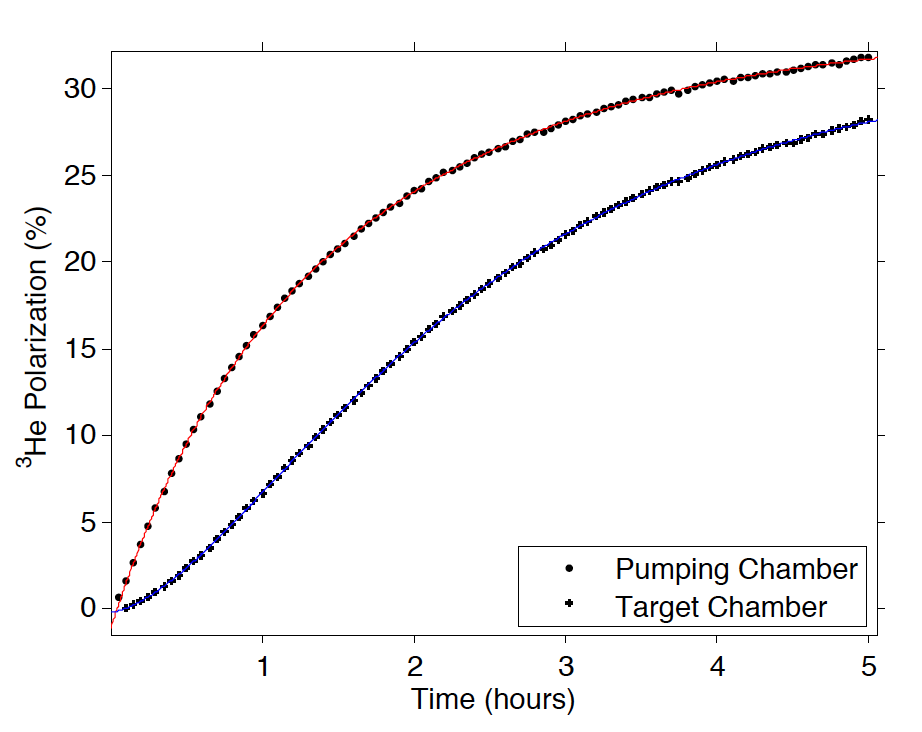
\includegraphics{BradySpinup.png}}
	\caption{{\bf $^{3}$He polarization as a function of time for both the pumping chamber and the target chamber. The top curve is the pumping chamber and the bottom curve is the target chamber.}}
	\label{BradySpinup}
\end{figure}

\subsubsection{Initial Spinup}

As shown in Fig.\ref{BradySpinup}, the early spinup behaviors of the pumping chamber and the target chamber are quite different. The initial part of the pumping chamber is almost linear but the target chamber shows a curved initial part. By performing a Taylor expansion on Eq.\ref{DoubleChamberSolution} we obtain the initial part of the spinup for both chambers:

\begin{subequations}\label{InitialSpinup}
	\begin{gather}
	P_{PC}(t)=\gamma_{se}P_{A}t-\frac{1}{2}\gamma_{se}P_{A}(\gamma_{se}+\Gamma_{PC}+d_{PC})t^{2}\\
	P_{TC}(t)=\frac{1}{2}\gamma_{se}P_{A}d_{TC}t^{2}
	\end{gather}
\end{subequations}

where $\gamma_{se}$ is the spin-exchange rate in the pumping chamber and $P_{A}$ is the alkali polarization. It's clear that the dominant term in $P_{PC}(t)$ is the linear term while the shape of $P_{TC}(t)$ is quadratic. 

The slope of the linear shape of initial spinup of the pumping chamber gives access to the product $P_{A}\gamma_{se}$ and fitting the initial spinup of the target chamber to a quadratic function provides the product $\gamma_{se}P_{A}d_{TC}$. The alkali polarization $P_{A}$ can be measured with the technique named Faraday Rotation, we then gain knowledge of the spin-exchange rate $\gamma_{se}$ and the diffusion rate $d_{TC}$.

\subsubsection{Spindown}

The spin relaxation rates in the pumping chamber and the target chamber are different due to geometry and other properties. The cell-average relaxation rate can then be written as

\begin{equation}
\langle \Gamma \rangle=f_{PC}\Gamma_{PC}+f_{TC}\Gamma_{TC}
\end{equation}

where $f_{PC}$ ($f_{TC}$) is the fraction of atoms in PC (TC); $\Gamma_{PC}$ ($\Gamma_{TC}$) is the average relaxation rate in PC (TC). When the cell is being pumped by laser, the pumping chamber is heated with hot air to create alkali vapor while the target chamber remains at the room temperature. The difference in temperature adds to the difference in relaxation rates. However, when trying to measure the life time (the inverse of the relaxation rate) of the cell, we typically keep the entire cell at room temperature and perform a "spindown" measurement. 

During a spindown, the cell starts with some polarization (normally as high as possible so we can obtain a more complete curve), and relaxes on its own while we take AFP measurements at a certain rate. Typically, the interval between measurements is anywhere between 30 mins and 2 hrs, depending on the lifetime of the cell. The rule of thumb is to take AFP frequently enough so the spindown curve has sufficient data points while not too often so the polarization relaxes much faster due to AFP losses. The $^{3}$He polarization relaxation can be described by

\begin{equation}\label{Spindown}
P(t)=P_{0}e^{-t/\tau_{true}}
\end{equation}

The true lifetime $\tau_{true}$ of the cell without relaxation due to AFP loss can be measured with two methods: the first is to take 5 AFP measurements consecutively with very short interval (normally around 3 minutes), the second is to perform several spindown measurements, each with a different interval. 

In the first method, because the lifetime of the cell is much longer than 3 minutes, we can safely attribute all losses to AFP measurements and extract the loss due to a single AFP $loss_{afp}$. The data values can then be corrected with the equation

\begin{equation}
S_{i}^{corrected}=S_{i}^{raw}/(1-loss_{afp})^{i}
\end{equation}

where $S_{i}^{corrected}$ is the corrected signal, $S_{i}^{raw}$ is the raw signal, i represents it is the $i$th measurement in the spindown, $loss_{afp}$ is the loss due to a single measurement. Fitting the corrected values to Eq.\ref{Spindown} gives the true lifetime $\tau_{true}$.

A simple example for the second method would be to perform one spindown with one-hour interval and another spindown with two-hour interval, the relaxation rates in these two spindowns are

\begin{subequations}
	\begin{equation}
	\frac{1}{\tau_{1hr}}=\frac{1}{\tau_{true}}+\Gamma_{AFP\_1hr}
	\end{equation}
	\begin{equation}
	\frac{1}{\tau_{2hr}}=\frac{1}{\tau_{true}}+\Gamma_{AFP\_2hr}
	\end{equation}
	\begin{equation}
	\Gamma_{AFP\_1hr}=2\times \Gamma_{AFP\_2hr}
	\end{equation}
\end{subequations}

where $\tau_{1hr}$ and $\tau_{2hr}$ are the lifetimes measured with taking AFP every 1 hour and every 2 hours, $\tau_{true}$ is the true lifetime of the cell without interference from measurements, $\Gamma_{AFP\_1hr}$ ($\Gamma_{AFP\_2hr}$)is the relaxation rate due to taking measurements every 1hr (2hr). We can then solve for $\tau_{true}$.

\subsection{AFP Loss}

The longitudinal spin relaxation rate due to static field inhomogeneities is

\begin{equation}
\frac{1}{T_{1}} = D\frac{|\nabla B_{x}|^{2}+|\nabla B_{y}|^{2}}{B_{0}^{2}}
\end{equation}

where D is the diffusion constant for the polarized spins, and is inversely proportional to the gas pressure. $B_{0}$ is the mean magnetic field along z axis. $B_{x}$ and $B_{y}$ are the x and y components of the magnetic field. However, when performing AFP measurement, the spins are exposed to a small oscillating RF field, the spin relaxation can be greatly accelerated under magnetic resonance conditions~\cite{PhysRevA.38.5092},

\begin{equation}
\frac{1}{T_{r1}} = \frac{8R^{4}}{175D}|\nabla \Omega_{z}|^{2}\sum_{n} \frac{175}{4(\chi_{1n}^{2}-2)(\chi_{1n}^{4}+r^{2}+r^{2}s^{2})(1+s^{2})}
\end{equation}

where R is the cell radius, D is the diffusion constant, $\Omega_{z}$ is the Larmor frequency of the holding field, $r=\frac{\omega_{r}R^{2}}{D}$, $s=\frac{\Omega_{0}-\omega}{\omega_{r}}$, the numbers $\chi_{1n}$ are the zeros of the derivatives of the spherical Bessel functions

\begin{equation}
\frac{d}{dx}j_{1}(x_{1n})=0~for~n=1,2,3...
\end{equation}

Since $r^{2}\gg \chi_{1n}^{4}$, and $\sum_{n}\frac{1}{\chi_{1n}^{2}-2}=\frac{1}{2}$~\cite{PhysRevA.37.2877},

\begin{equation}
\frac{1}{T_{r1}}=\frac{R^{4}|\nabla\Omega_{z}|^{2}}{r^{2}(1+s^{2})^{2}D}=\frac{|\nabla B_{z}|^{2}D}{B^{2}(1+s^{2})^2}
\end{equation}























\section{Electron Paramagnetic Resonance}


\chapter{Lorem Ipsum}
\label{chap:ch4_abbr}
Now, for your reading pleasure, some \textsl{Lorem ipsum}, courtesy
of:

\chapter{Development of Hybrid Targets}
\label{chap5}

\section{Overview}

Electron scattering experiments at JLab have traditionally used $^{3}$He targets made of glass due to the compatibility with spin-exchange optical pumping, the capability to be shape into desired geometries through glass blowing, and the excellent nuclear spin relaxation properties. The borosilicate glass Pyrex had been the glass of choice prior to the discovery that the much less permeable aluminosilicate glass generally provides longer spin-relaxation time. The most recent targets were thus composed entirely of the aluminosilicate glass GE180.

After the 12 GeV upgrade, JLab plans to run experiments with much higher electron beam currents. The maximum current used before the upgrade was 15$\mu$A, while future experiments will be run at up to 60$\mu$A. We believe an all-glass target cell might survive long enough for an experiment with 30$\mu$A, but it is unlikely to survive at 60$\mu$A. A natural solution would be to replace the thin glass window (where electron beam enters and exits the target cell) with a material with higher strength and good spin-relaxation properties. 

Deninger~\emph{et al.} from the Mainz group showed relaxation time of various metal surfaces: Mg (6 h), Al (6 h), Zn(12 h) etc. Gold caught our attention in particular, because it has a relatively long relaxation time of 20 h. This relaxation time was measured by coating the glass surface with gold, thus the area of gold surface was much larger than what will be needed for target windows. In addition, while the coating process made sure of the chemical purity, it did not make effort in ensuring the microscopic smoothness, which means the surface area was further increased. In light of this, our group have tested 19 cells with various geometries and materials, most of which incorporate a OFHC (oxygen-free high thermal conductivity) copper tube with gold coating. OFHC copper was chosen as the substrate in most cases because of its structural strengths and the familiarity with manufacturers. Towards the end of my work, we achieved a 15.6 h relaxation time with a Pyrex cell that had a 5'' long by 1'' gold coated copper tube attached horizontally. By extrapolating the relaxation rate due to gold surface from this result, we believe the relaxation rate introduced by small metal windows in a target cell will be less than 1/135 h$^{-1}$. To the best of our knowledge, our group was the first to have proved the potential of incorporating metal to target cells in the presence of alkali vapor.

\section{Wall Relaxation of $^{3}$He}

\subsection{Relaxation on Glass Surfaces}

Fitzsimmons and Walters have studied surface-induce spin-lattice relaxation times as a function of temperature for $^{3}$He gas in glass containers~\cite{PhysRev.179.156}. There are mainly two categories of wall relaxation mechanisms: $^{3}$He adsorption on the glass surface and the permeation of $^{3}$He into glass. The latter mechanism can be greatly reduced by using impermeable aluminosilicate glass such as GE180. 

Timsit and Daniels~\cite{Timsit} then studied surface relaxation on a great number of common materials and presented a phenomenological model to describe the relaxation processes.For permeable glasses, the relaxation is determined by absorption of gas in the surface layer of the glass and by the paramagnetic impurity content of the glass. The surface adsorption of $^{3}$He near paramagnetic sites on the walls also contributes to the nuclear relaxation. Relaxation due to absorption for permeable glasses will be discussed first below.

The diffusion coefficient $D$ of a noble gas in a glass can be calculated with the following equation:
\begin{equation}\label{D}
D=D_{0}e^{-Q_{d}/kT}
\end{equation}
where $Q_{d}$ is the activation energy for diffusion and $D_{0}$ is a constant. The diffusion coefficient can also be expressed with the mean diffusion jump distance of $^{3}$He atom in the glass $\langle\Delta r\rangle$ as:
\begin{equation}
D=\frac{\langle\Delta r\rangle^{2}}{6\tau}
\end{equation}
where $\tau$ is the mean time between diffusion jumps
\begin{equation}\label{residence_time}
\tau=\tau_{0}e^{E_{dif}/kT}
\end{equation}
where $\tau_{0}=\langle\Delta r\rangle^{2}/6D_{0}$.

Let $n_{g}$ be the number of atoms dissolved in the surface layer of mean thickness $\langle\Delta r\rangle$, the rate at which $^{3}$He atoms enter and leave the surface layer of the glass is then $n_{g}/6\tau$. $n_{g}$ should be proportional to the solubility $S$ of $^{3}$He in the glass, so for a spherical cell
\begin{equation}\label{absorption_ng}
n_{g}=\frac{6NkT\langle\Delta r\rangle S}{d}
\end{equation}
where d is the diameter of the cell, N is the total number of free $^{3}$He atoms.

The intrinsic relaxation time $T_{i}$ is longer than $\tau$, the time it takes for $^{3}$He to leave the $\langle\Delta r\rangle$ layer, for most trapping sites in the glass. However, $T_{i}$ for a paramagnetic site is shorter than $\tau$, thus will completely relax the nuclear spin of a $^{3}$He atom. The relaxation time of $^{3}$He in permeable glass cells is controlled by absorption of the atoms in the surface layer at paramagnetic sites. The average nuclear relaxation time of a $^{3}$He trapped in the glass close to a Fe$^{3+}$ ion (one common type of paramagnetic impurity in glass) is~\cite{Abragam}:
\begin{equation}
\frac{1}{T_i}\approx\frac{3}{5}\frac{\mu_{He}^{2}\mu_{B}^{2}g^2}
{\hbar^2b^6}\frac{T_{Fe}}{1+\omega_0^2T_{Fe}^2}
\end{equation}
where $\mu_{He}$ is the nuclear dipole moment of $^{3}$He, $\mu_B$ is the Bohr magneton, g is the g factor of the Fe$^{3+}$ ($^{6}S_{5/2}$) ion, and b is the distance between the spins. Taking b as 1 $\mathring{A}$ and g as 5.9~\cite{Kittel}, $T_i$ is $\sim10^{-11}$ s, which is 10 times smaller than the shortest $\tau$.

Even a small amount of paramagnetic impurities among the trapping sites in the glass can provide dominating contribution on the $^{3}$He spin relaxation. Assuming during the random walk of $^{3}$He atom in the glass, there are on average $\beta$ atoms in its vicinity, and atom fraction of paramagnetic impurities is $N_{impurity}$, the relaxation time due to absorption is if $T_i\ll\tau$:
\begin{equation}\label{T_ab}
T_{ab}=\frac{6N\tau}{\beta N_{Fe}n_g}
\end{equation}

For impermeable glasses such as GE180, the relaxation rate due to absorption into the glass walls is typically negligible. The dominating relaxation mechanism here is adsorption of $^{3}$He on the glass wall in vicinity of a paramagnetic site.

The sticking time $tau_s$ is given by Frenkel's Law:
\begin{equation}\label{sticking_time}
\tau_s=\tau_{s0}e^{E_{ad}/kT}
\end{equation}
where $\tau_{s0}$ is on the order of $10^{-13}$ s for most solid surfaces~\cite{Frenkel}, $E_{ad}$ is the adsorption energy. At room temperature, we have $\tau_s\sim\tau_{s0}\sim 10^{-13}$ s. The number of atoms hitting the wall per unit time and unit area is given by $\frac{1}{4}n\bar{v}$, where n is the number density of $^{3}$He gas and $\bar{v}$ is the mean velocity. For a spherical cell with diameter d, the number of atoms adsorbed on the wall is
\begin{equation}\label{adsorption_ng}
n_{g}'=\frac{3N\bar{v}\tau_s}{2d}
\end{equation}

The intrinsic relaxation time $T_i'$ of a $^{3}He$ near a paramagnetic site on the wall is much longer than the sticking time $\tau_s$. The average number of collisions required to depolarize $^{3}$He is $T_i'/\tau_s$, thus the relaxation time due to adsorption is
\begin{equation}\label{T_ad}
T_{ad}=\frac{NT_i'}{N_{impurity}n_g'}
\end{equation}

The total relaxation rate is the sum of that due to adsorption and absorption (for permeable glasses):
\begin{equation}
\frac{1}{T_{wall}}=\frac{1}{T_{ad}}+\frac{1}{T_{ab}}
\end{equation}

Substitute Eq.~\ref{residence_time},~\ref{absorption_ng} into Eq.~\ref{T_ab} and Eq.~\ref{sticking_time},~\ref{adsorption_ng} into Eq.~\ref{T_ad}, the wall relaxation rate can be written as
\begin{equation}
\begin{split}
\frac{1}{T_{wall}}=&\frac{\beta N_{impurity}kT\langle\Delta r\rangle S}{d\tau_0}e^{-E_{dif}/kT}\\
&+\frac{3N_{impurity}\bar{v}\tau_{s0}}{2dT_i'}e^{E_{ad}/kT}
\end{split}
\end{equation}

According to the above equation, both the diffusion-induced and the surface-induced relaxation rates are proportional to the surface-volume ratio of the cell, \emph{i.e.} to the inverse of the cell diameter $d$. Thus it is useful to describe the surface relaxation properties with a physical quantity $rho$, which is commonly referred to as the "relaxivity". The relaxivity is independent of cell geometry and is related to the wall relaxation rate $1/T_{wall}$, the surface to volume ratio $A/V$ by the following equation:
\begin{equation}
1/T_{wall}=\rho A/V
\end{equation}

Fitzsimmons~\emph{et al.}~\cite{PhysRev.179.156} found by using impermeable aluminosilicate glass, the relaxation due to absorption can be greatly reduced thus increasing the total relaxation time. Heil~\emph{et al.} reported~\cite{PhysRevA.201.337} glass cells that were internally coated with metallic films provided even longer relaxation time. Ce was one of the metals that greatly reduced wall relaxation rate as it blocks $^{3}$He atoms from diffusing into the glass walls and it also has a low adsorption energy which leads to very short sticking time. For SEOP (Spin-Exchange Optical Pumping), we automatically profit from the Rb film which covers the inner surface of the pumping chamber. Similarly, another way to eliminate relaxation due to absorption is to coat the inner surface with sol-gel~\cite{solgel}. It is a mixture of aluminum nitrate nonahydrate $Al(NO_3)_39H_2O$, ethanol and deionized water. The sol-gel coating also improves relaxation time by blocking $^{3}$He atoms from diffusing into the glass.

\subsection{Relaxation on Metal Surfaces}

Since $^{3}$He gas does not diffuse into metals~\cite{barrer}, the relaxation is purely due to surface effects. However, the surface-induced relaxation on metal surfaces is not yet well understood. There are two additional relaxation mechanisms with metal surfaces compared to those for glass. First mechanism is the depolarization of $^{3}$He nuclei near the metal surface by oscillating magnetic field from eddy currents induced by the movement of these same nuclear dipoles. Smythe~\cite{Smythe} derived the magnetic field generated in pace by eddy current induced in a metal sheet by a moving magnetic dipole using the method of images. Timsit~\emph{]et al.}~\cite{Timsit} estimated the relaxation due to eddy currents using the same method:
\begin{equation}
\frac{1}{T_m} = \frac{3\times 10^{-4}}{\pi} \frac{\mu_{He}^4}{\bar{v}r_{0}^{4}\hbar^{2}}\frac{A_p}{d^3}
\end{equation}
where $\bar{v}$ is the mean velocity of atoms, $r_0$ is the closest distance of the nucleus to the metal surface, d is the cell diameter, $A_p$ is the area. According to Timsit~\emph{et al.}, $T_m$ is on the order of $10^{16}$ s if $r_0=1\mathring{A}$ and $A_p = 9.2cm^2$. Even though the area of the cell is usually much larger and other parameters may take different values, but it should still remain true that the relaxation rate of $^{3}$He due to eddy currents can by safely neglected.

The second additional mechanism that contributes for relaxation of $^{3}$He adsorbed on the metal surfaces is the Korringa scattering. Nuclear spin relaxes when the nucleus interacts with conduction electrons in the metal, where the an electron flips its spin and the spin state of the nucleus changes. The Pauli exclusion principle states that the interaction is only allowed when the final state the electron jumps to is initially unoccupied. Thus according to Fermi statistics, only electrons with energy close (approximately within kT) to the Fermi energy level can participate in such interactions. Slichter~\cite{Slichter} has derived the Korringa relaxation rate in metal to be:
\begin{equation}
\frac{1}{T_K}=\frac{(4\pi)^6}{9h^7}(g_s\mu_B \frac{\mu_K}{K})^2 \eta^4m^3\epsilon_F kT
\end{equation}

To calculate the total Korringa relaxation rate due to metal surface, one needs to consider the overlapping of wave functions of the conduction electrons and the nuclei of adsorbed $^{3}$He atoms in the vicinity of the metal surface. Nelson~\cite{NelsonThesis} derived the total surface Korringa relaxation as:
\begin{equation}
\frac{1}{T}=\frac{1}{T_K}\frac{S}{V}\int_{0}^{\infty} f\left(l\right)^2 e^{-U\left(l\right)/kT}dl
\end{equation}
where S and V are the surface area of the metal and total volume of the cell, respectively, $U\left(l\right)$ is the atom-surface potential with the edge of the metal taken as $l=0$, $f\left(l\right)$ is the fractional density of conduction electrons outside the surface. Nelson further used the work function of the metal to estimate $f\left(l\right)$, and assumed a van der Waals form for $U\left(l\right)$. His calculations suggest that the Korringa relaxation times for $^{3}$He on various metal surfaces should be thousands of years, including the metal of interest for our studies, gold.

If eddy currents and Korringa relaxation are the only surface relaxation mechanisms, we would have very long lifetime for our test metal cells. Unfortunately, our series of studies have shown relaxation times to be between a few hours and 16 hours most of the time, for which both aforementioned relaxation mechanisms can be safely neglected. Although the dominating relaxation mechanism is still not well understood and significantly faster than those we have better understanding about, the results of our studies are still promising, as they suggest the extra relaxation rate due to use of small metal end windows should still be small enough and allow future experiments to run at 60$\mu$A electron beam current.

\section{Test Cell Fabrication}

\subsection{Overview}

In order to study the relaxation rate due to metal surface, we have created and tested 19 cells so far, most of which contains a metal tube. The metal tubes are 5'' in length and 1'' outer diameter, 3'' of glass tubes are attached to both ends via Houskeeper seal. The total area of the metal surface is 101.3 $cm^2$, and is far larger than what will be for metal end windows. This large geometry is chosen to intentionally increase the relaxation rate for studying. This particular design of metal tube is also favored for the convenience of manufacturing, as we were expecting a large number of test cells to be studied and any design that saves time could potentially mean a much shorter test time before we determine the final design.

The making of these test cells usually include five steps (except control cells with pure glass and cells without gold coating):

1. Larson Electronic Glass~\cite{Larson} provides us a glass-to-metal-to-glass tube that uses Houskeeper seal to attach glass to metal

2. The machine shop in the physics department of University of Virginia then mechanically polishes the inside of the metal tube.

3. Able Electropolishing electropolishes the metal tube.

4. Epner Technology Inc. electroplates the metal tube with gold.

5. Mike Souza at Princeton University, our glass blower, resizes the glass from stock material and makes the final cell with our desired dimensions and attaches the metal tube to the glass cell. The resizing is for removing micro-fissures from the glass surface and reducing wall relaxation rates~\cite{Cates1993}.

Each step will be described below.

\subsection{Glass-to-Metal Seal}

Larson Electronic Glass made the glass-to-metal-to-glass tubes for us, Fig.~\ref{metal_tube} is a picture of one the tubes used in our tests. The glass-to-metal seal used by Larson is known as the Houskeeper seal~\cite{Houskeeper}. The outside of the copper tube is machined down to a knife edge and is wetted with glass. The edge of copper is usually heated before covering with glass. The heating process creates a thin layer of crimson-color copper oxide as can be seen in Fig.~\ref{metal_tube}. Houskeeper seals were originally used for vacuum, we checked each seal down to the $10^{-10}mbar\cdot l/s$ level. To make sure these seals will survive the high pressure JLab experiments, we also tested the integrity of them under up to 15 atm for extended period of time.

\begin{figure}[t!]
	\centering
	\resizebox{0.91\textwidth}{!}{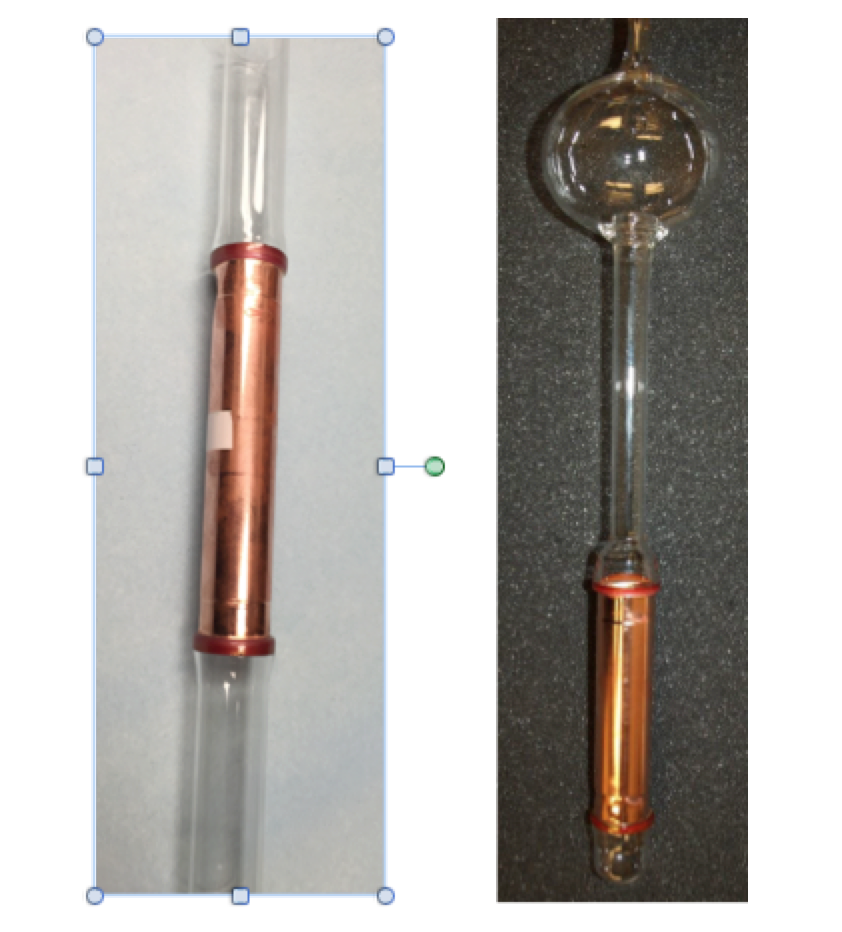
\includegraphics{metal_tube.png}}
	\caption{{Shown is a glass-to-metal-to-glass seal. The metal tube is 5'' long by 1'' outer diameter. The glass is wetted onto the knife-edge of copper on both ends.}}
	\label{metal_tube}
\end{figure}

The copper used in our tests is OFHC (oxygen-free high thermal conductivity) copper. In the earlier stage of our tests, OFHC copper was attached to the Pyrex glass, in which case a direct connection could be made. For the later tests where we were moving closer to the final goal of using metal end windows with the impermeable aluminosilicate glass GE180, a transition glass between OFHC copper and GE180 had to be used. The coefficient of expansion for GE180 glass is not compatible for making a direct seal with OFHC copper, thus Corning 7052 Kovar sealing glass was used as the transition. The two materials connected by a seal should have similar coefficients of expansion, the 7052 Kovar sealing glass serves as an intermediate material to bridge the gap between OFHC copper and GE180. The other type of metal used in our glass-to-metal seals was titanium, for which only Pyrex was used.

\subsection{Mechanical and Electropolishing}

The mechanical polishing is done by our machine shop in the department. A wire brush attached to a lathe was placed inside the tube while the lathe spun. This first-step polishing produced a relatively smooth surface in preparation for the following electropolishing process.

After the tubes were mechanically polished by the machine shop, they were sent to Able for electropolishing. The tube serves as the cathode, whihc is immersed in a temperature-controlled bath of electrolyte and connected to the positive terminal of a DC power supply, while the cathode is the attached to the negative terminal. During electropolishing, the polarized film is subjected to combined effects of gassing (oxygen) that occurs with electrochemical metal removal, saturation of the surface with dissolved metal and the agitation and temperature of the electrolyte. Metal on the surface is oxidized and dissolved in the electrolyte, the microscopic high points on the surface dissolve faster than the rate of attack on the rest parts of the surface, which provides a smoothing effect. As a result, the electropolishing process removes a thin layer of metal (about 20 $\mu m$ for our tubes), leaving a microscopically smooth and featureless surface. By contrast, even a fine mechanically polished surface will still show smears and other directionally oriented patterns or effects\cite{Electropolishing}. Fig.~\ref{Electropolishing} shows a diagram of the polishing process and its smoothing effect.

\begin{figure}[t!]
	\centering
	\resizebox{0.91\textwidth}{!}{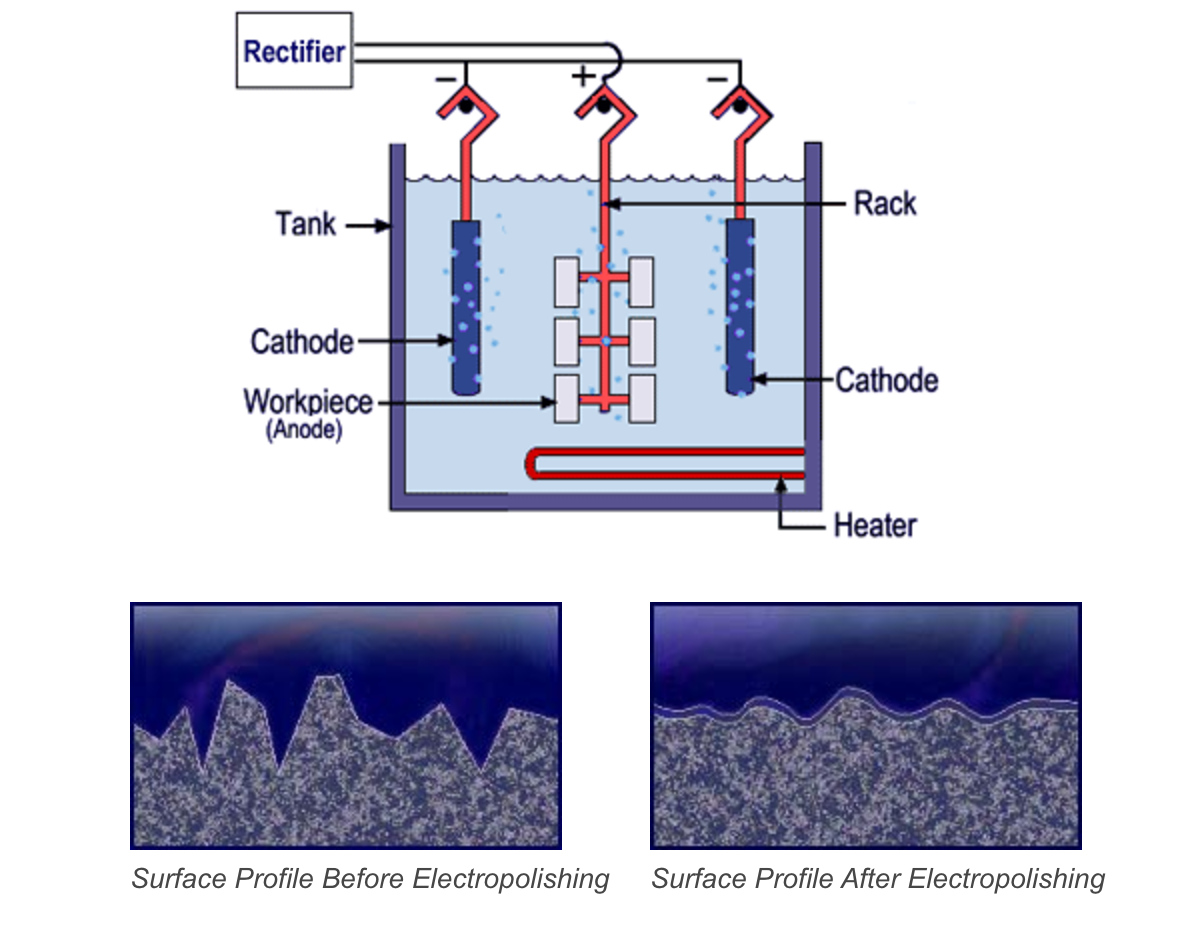
\includegraphics{Electropolishing.png}}
	\caption{{Electropolishing~\cite{Electropolishing}}}
	\label{Electropolishing}
\end{figure}

\subsection{Electroplating}

As stated earlier, because of the good lifetime reported by Deninger~\emph{et al.}, gold was plated on the inner surface of the OFHC copper and titanium tubes. Epner Technology Inc. handled the electroplating for us. Electroplating is the reverse process of electropolishing. When electric current passes through the electrolyte, the electrolyte splits up and some of the desired metal atoms it contains are deposited in a thin layer on top of the electrodes. Nickel an chromium are two common undercoatings used for electroplating, however, they are both ferromagnetic and can't be used for us as they would introduce additional spin relaxations. As a result, Epner used a copper strike to improve the durability of gold coating. A 5 $\mu m$ layer of gold was subsequently electroplated on the inner surface of the tubes. Fig.\ref{gold_coating} shows a comparison of a OFHC copper tube with gold-coating and a tube without any coating. 

\begin{figure}[t!]
	\centering
	\resizebox{0.91\textwidth}{!}{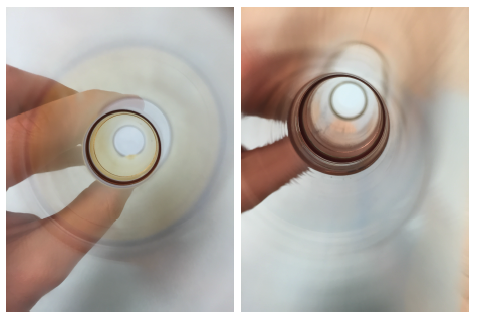
\includegraphics{gold_coating.png}}
	\caption{{Shown left is the inner surface of a gold coated OFHC copper tube. Shown right is a OFHC copper tube without coating.}}
	\label{gold_coating}
\end{figure}

\subsection{Final Assembly of the Cell}

After the tubes were coated and shipped back to us and leak checked one more time, they were cleaned with our ultrasonic cleaner. Fig.~\ref{ultrasonic_cleaner} shows the setup of the cleaning process. We cleaned the impurities on the surfaces of the tubes with ethanol, deionized water and methanol for thirty minutes each. As shown in the figure, a beaker containing the chemical solution and the tubes were placed in water bath inside the ultrasonic cleaner. Because of the dimensions of the cleaner and the beaker, we cleaned one end of the tubes first then flipped them to clean the other end before switching solution.

\begin{figure}[H]
	\centering
	\resizebox{0.4\textwidth}{!}{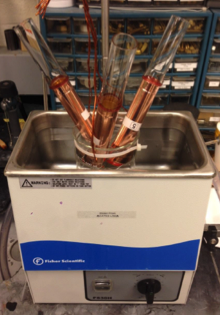
\includegraphics{ultrasonic_cleaner.png}}
	\caption{{Ultrasonic cleaner with 3 tubes being cleaned.}}
	\label{ultrasonic_cleaner}
\end{figure}

The test tubes were then shipped to our glassblower Mike Souza at Princeton University. All glass was reblown to the right size to reduce micro-fissures which would lead to high relaxation rate. The test tube was spliced with transfer tube and a pumping chamber. A string (see Fig.~\ref{string}) which would be used for cell filling was also made at Pricenton. Traditionally, a pure glass cell would be placed entirely in a oven for annealing. A cell made with GE180 would go through a five-minute ramping time to 780$^{\circ}C$, stay at 780$^{\circ}C$ for five minutes and slowly cool down to room temperature for at least 5 hours~\cite{DanThesis}. A Pyrex cool would be annealed in the exact same way except the highest temperature would be 565$^{\circ}C$. However, most our test cells could not have been annealed in the same way because of the glass-to-metal seal. Had we expose the seal to high temperature for long period of time, gold atoms might have migrated into the metal substrate and the seal might even break. Thus the metal tubes were attached to the rest of the glass parts after the pure glass parts were annealed. The finished cells together with glass strings were shipped to us.

\begin{figure}[t!]
	\centering
	\resizebox{0.91\textwidth}{!}{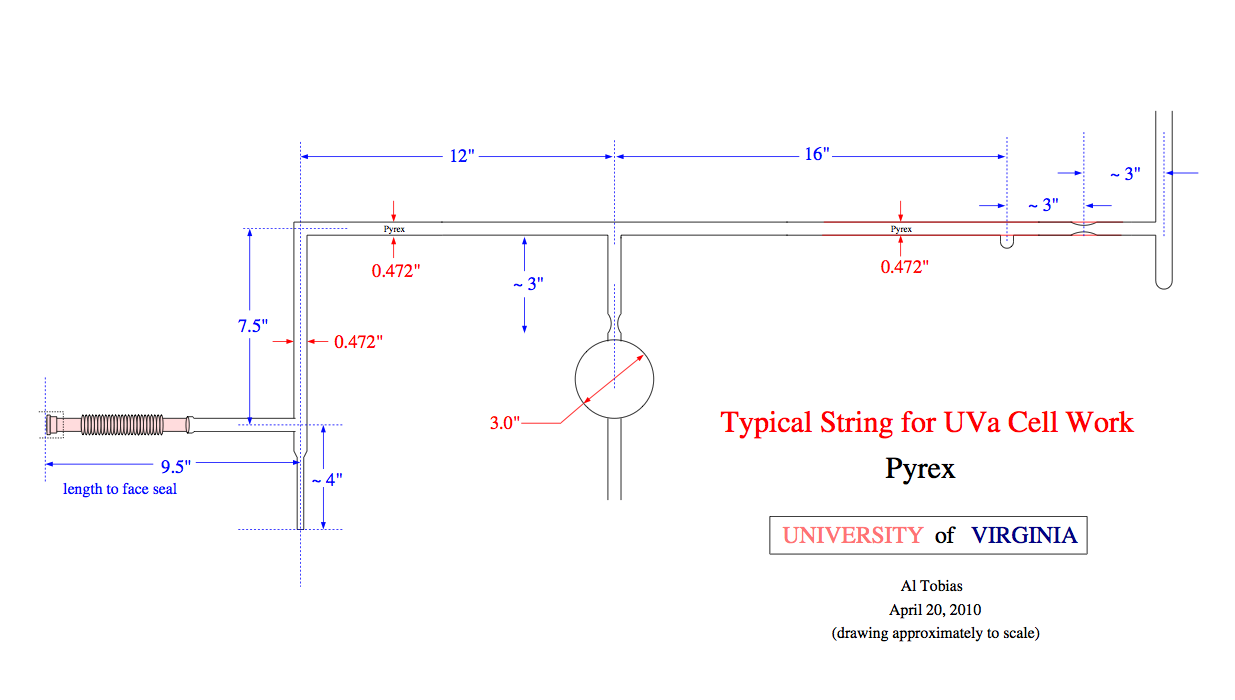
\includegraphics{string.png}}
	\caption{{Shown is the design of a typical string for our test cells.}}
	\label{string}
\end{figure}

\section{Cell Fill Procedure}

The details of cell fill was described thoroughly by Matyas~\cite{DanThesis}, I will briefly cover the process for the sake of completeness.

\subsection{Cell Fill Preparation}

Although the actual cell fill work only took less than a day, the preparation that led to the fill usually took 10-15 days. The string, cell and the retort (see Fig.\ref{}) were spliced together and attached to our homemade gas system through the bellows. a pre-scored ampoule of alkali metal was dropped from the top the of the retort.  Fig.~\ref{cell_gas_system} is a diagram of the string, cell and retort all connected together. 

\begin{figure}[t!]
	\centering
	\resizebox{0.91\textwidth}{!}{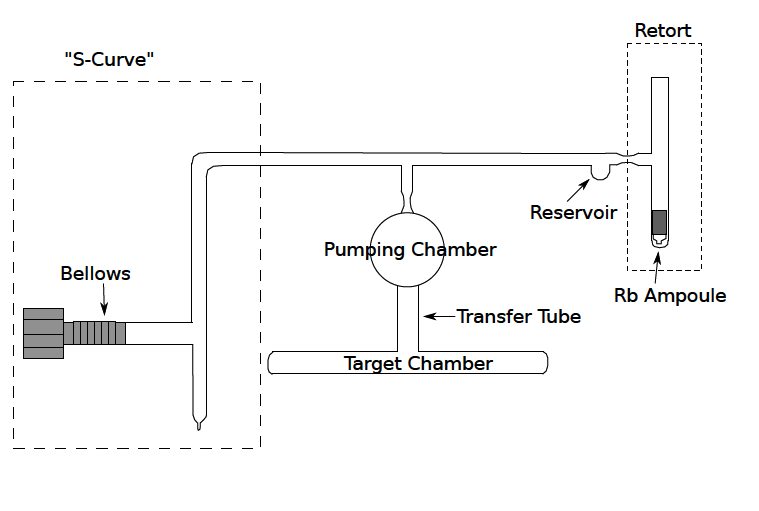
\includegraphics{cell_gas_system.png}}
	\caption{{A diagram of a Pyrex string with a cell and a retort attached while connected to the gas system through the bellows. Adapted from Matyas~\cite{DanThesis}.}}
	\label{cell_gas_system}
\end{figure}

The entire system was first rough-pumped down with a mechanical pump, and then kept being pumped by a diffusion pump to even lower vacuum. After the system was pumped for a few days and alkali metal was added in the system, we would keep pumping the system with the diffusion pump for roughly a week. To prevent the hot oil in the diffusion pump from going up into the gas system and the cell, a cold trap above the diffusion pump was filled every day with liquid nitrogen. "Flamebakes" were also performed 2-3 times a day during the one-week pumping period. A methane-oxygen torch was used to gently bake on the glass parts in the flamebakes. The bake should start from the retort which the farthest away from the diffusion pump, and move slowly towards the bellows, so the impurities chased off the inner surfaces can be "swept" towards the pump leaving as few impurities behind as possible. The alkali metal was typically melted on the second or third flamebake and should be melted during each of the remaining flamebakes. On the day before the fill, alkali metal was melted and chased into the pumping chamber.

\subsection{Cell Fill}

The first thing on the fill day was to make sure pump all portions of the gas system to vacuum and selectively back fill some parts with appropriate gases (either N$_2$ or $^{3}$He) to minimize outgassing. The gas filled into the cell should always be cleaned during the path to the cell. Earlier test cells were filled with the noble gas purifier while the later cells were done with a homemade cold trap.

The homemade cold trap consisted of a copper tubing placed inside box-shaped Dewar. The Dewar was filled with liquid nitrogen when filling N$_2$ and liquid helium when filling $^{3}$He, so impurities in the gas were frozen in the copper tubing. Temperature inside the dewar was monitored with two silicon diodes to determine whether copper tubing was fully submerge in the cold liquid.

The volume of the cell was also determined during the fill process. A Baratron pressure gauge was used to measure a calibrated volume (CV) of 992.9 cc. 300 Torr of gas was filled into the calibrated volume, then the valve on CV was closed and any gas outside of CV was pumped away. Next the gas kept in CV was let out into the fill gap between CV and the string while monitoring pressure with the Baratron gauge, thus the volume of the cell could be calculated with ideal gas law.

Around 70 Torr of nitrogen was put into the cell before filling $^{3}$He. To prevent nitrogen from escaping the cell while filling $^{3}$He, the string valve was kept closed until $^{3}$He pressure in fill gap rose well above 70 Torr. A total gas pressure of just under 760 Torr (1 atm) was reached. This target pressure was chosen because when the connection between the cell and the string was melted, the atmospheric pressure would collapse it and seal the cell for us. All cells except Kappa1 contained pure rubidium, while Kappa1 was contained 5:1 alkali mixture of potassium to rubidium.

\section{Experimental Procedure}

All cells incorporated metal were tested with Pulse NMR as it is only affects a small region of the cell and minimizes influences from eddy current in the metal tubes. Kappa1 was a simple spheric and pure GE180 cell, which was built to rule out the possibility that the melt of GE180 our cells had been made of was bad. Because of its lack of metal and lack of convenient places to wrap pickup coils on, Adiabatic Fast Passage was used to test Kappa1. Both PNMR and AFP were discussed in a general way in chapter 3, I will add on to the discussions with more specific experimental setups for this study.

\subsection{Pickup Coils}

In a AFP measurement, pickup coils are placed next to the side windows of the oven. However, the same setup proved to be more difficult for us to receive high-quality PNMR signals. To still keep the pickup coils outside of the oven, we manually wrap a solenoid coil on the transfer tube of test cells where it is approximately 2'' below the bottom of the oven. These coils were made with 40-50 turns of AWG 20 copper wire. Because of the off-center positions of the pickup coils, inhomogeneities were significant enough to affect FID signals, gradient coils were used to cancel the inhomogeneities.

\subsection{Gradient Coils}

Inhomogeneities were canceled to the best we could empirically with three sets of gradient coils. Each set of gradients coils consists of two oppositely wound coils separated by a distance $d$, this particular type of coils are referred to as "Maxwell coils". The setup is very similar to that of Helmholtz coils, except the opposite direction of currents and the larger optimum separation $d=R$, where $R$ is the radius of the coils. The opposite direction is to cancel out the magnetic field at the center, and the optimum separation makes the first four leading terms in the Taylor expansion zero\cite{Callaghan}. Fig.\ref{gradient_coils} shows the coil orientations. The z axis is defined to be aligned with the direction of the holding field while x and y axes are in the transverse plane. The direction of coil axis is then defined by the angle $\theta$ and $\phi$, where $\theta$ is with respect to the z axis and $\phi$ is the azimuthal angle in the x-y plane.

\begin{figure}[t!]
	\centering
	\resizebox{0.91\textwidth}{!}{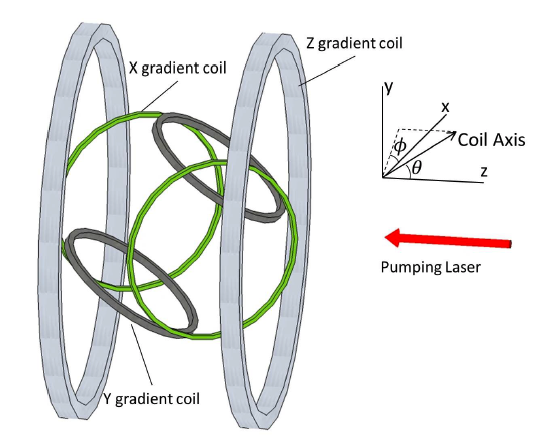
\includegraphics{gradient_coils.png}}
	\caption{{Diagram of the coils. Adopted from Zheng~\cite{YuanThesis}.}}
	\label{gradient_coils}
\end{figure}

The magnetic field at the center is given by\cite{PhysRevA.37.2877}

\begin{equation}\label{gradient}
\begin{split}
\nabla\boldsymbol{B}(\theta, \phi)
&=\begin{bmatrix}
\partial B_x/\partial x & \partial B_y/\partial x & \partial B_z/\partial x \\
\partial B_x/\partial y & \partial B_y/\partial y & \partial B_z/\partial y \\
\partial B_x/\partial z & \partial B_y/\partial z & \partial B_z/\partial z
\end{bmatrix}\\
&=3\kappa I
\begin{bmatrix}
sin^2\theta cos^2\phi-\frac{1}{3} & sin^2\theta sin\phi cos\phi & sin\theta cos\theta cos\phi \\
sin^2\theta sin\phi cos\phi & sin^2\theta sin^2\phi-\frac{1}{3} & sin\theta cos\theta sin\phi \\
sin\theta cos\theta cos\phi & sin\theta cos\theta sin\phi & cos^2\theta-\frac{1}{3}
\end{bmatrix}
\end{split}
\end{equation}
where the calibration constant $\kappa$ is:

\begin{equation}
\kappa = \frac{3\pi n R^2 d/2}{5(d^2/4+R^2)^{5/2}}G\,cm\,A^{-1}
\end{equation}

The most important terms in Eq.\ref{gradient} are those related to $B_z$: $\partial B_z/\partial x$, $\partial B_z/\partial y$ and $\partial B_z/\partial z$. The orientations of the gradient coils can be chosen such that each of the three sets of coils controls one of the aforementioned terms. This "magic angle" $\theta_m$ is given by

\begin{equation}
\theta_m = cos^{-1}1/\sqrt{3}=54.7^{\circ}
\end{equation}

For $\theta=\theta_m$ and $\phi=0$ the gradient tensor is

\begin{equation}
\nabla\boldsymbol{B}(\theta_m, 0)=\kappa I
\begin{bmatrix}
1 & 0 & \sqrt{2}\\
0 & -1 & 0 \\
\sqrt{2} & 0 & 0
\end{bmatrix}
\end{equation}

For $\theta=\theta_m$ and $\phi=\pi/2$ we have

\begin{equation}
\nabla\boldsymbol{B}(\theta_m, 0)=\kappa I
\begin{bmatrix}
-1 & 0 & 0\\
0 & 1 & \sqrt{2}\\
0 & \sqrt{2} & 0
\end{bmatrix}
\end{equation}

Finally, for the z gradient coil we have

\begin{equation}
\nabla\boldsymbol{B}(\theta_m, 0)=\kappa I
\begin{bmatrix}
-1 & 0 & 0\\
0 & -1 & 0\\
0 & 0 & 2
\end{bmatrix}
\end{equation}

Our gradient coils were built by Zheng~\cite{YuanThesis}. The separations were do not follow the optimum condition $d=\sqrt{3}R$ due to spatial limitations. The dimensions of the gradient coils are shown in Table~\ref{gradient_coils_table}.

\begin{center}
	\begin{tabular}{ | c | c| c| c | }
		\hline
		& turns & radius & separation \\ \hline
		x & 42 & 33 cm & 64 cm \\ \hline 
		y & 100 & 28 cm & 56 cm \\ \hline
		z & 8 & 66 cm & 66 cm \\
		\hline
	\end{tabular}
\end{center}\label{gradient_coils_table}

\subsection{Laser Setup}

In earlier stage of the study, narrow-band Commet laser from Newport was used. Each Commet laser provides roughly 20 W power, the optical fibers were combined through a combiner which requires water cooling if multiple lasers are on at the same time. In later studies, single Raytum laser was used instead as it can provide much higher power. Both Commet laser and Raytum laser have around 0.2 nm FWHM (full width at half maximum).

Fig.~\ref{optics} shows a diagram of the optics used for SEOP (spin-exchange optical pumping). After the combiner, laser was focused by two lenses L1 and L2 such that the power spread enough to not damage the polarizing cube and was focused to an appropriate size at the cell position. The polarizing cube separated the beam into two beams with orthogonal linear polarizations. The beam with polarization parallel to this plane went through the cube, and the other beam with polarization perpendicular to the plane was reflected. The reflected beam went through a QWP (quarter wave plate), reflected at a mirror, went through the QWP one more time. Its polarization was changed to be parallel to this plane at this point and went through the cube. This beam is referred to as the "main beam" as it is ideally aligned with the holding field. The beam that went through the cube the first time was sent towards the oven by a mirror. Because of the small angle relative to the main beam, this is called the "skew beam". Both the main beam and the skew beam went through QWP before arriving at the oven window and were turned to circular polarization in the same direction.

\begin{figure}[t!]
	\centering
	\resizebox{0.91\textwidth}{!}{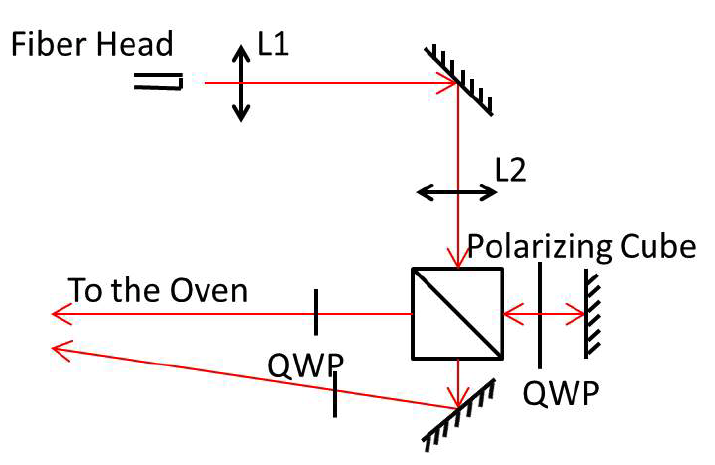
\includegraphics{optics.png}}
	\caption{{Optics for spin-exchange optical pumping. Adopted from Zheng~\cite{YuanThesis}.}}
	\label{optics}
\end{figure}

\subsection{}


\chapter{Conclusions}
\label{chap:conclusions}
That's all folks!


\addcontentsline{toc}{chapter}{Bibliography}
\bibliography{ref}


% \appendix
% \chapter{Appendix title}
\label{apdx:somelabel}
This is Appendix~\ref{apdx:somelabel}.

You can have additional appendices too
(\emph{e.g.}, \texttt{apdxb.tex}, \texttt{apdxc.tex}, \emph{etc.}).
If you don't need any appendices, delete the appendix
related lines from \texttt{thesis.tex} and the file names
from \texttt{Makefile}.

	
\end{document}
